\documentclass[
    12pt,               
    a4paper,            
    twoside,                  
    chapterprefix=false,
    captions=tableheading,
    headings=optiontohead % optional \chapter[...] argument sets the running head only; ToC keeps the full descriptive title
]{scrreprt}

% --- LANGUAGE & FONT ---
\usepackage[T1]{fontenc}
\usepackage[british]{babel}   % british: matches the British spelling used throughout
\usepackage[scaled]{helvet}         
\renewcommand{\familydefault}{\sfdefault} 
\usepackage{setspace}
\setstretch{1.2}
\setlength{\parindent}{0pt} % Sets paragraph indent to 0

% --- PAGE LAYOUT (Word guidelines) ---
\usepackage[
    inner=3cm, 
    outer=2cm, 
    top=2.5cm, 
    bottom=3cm, 
    bindingoffset=0cm
]{geometry}

% --- SPACING FOR HEADINGS ---
\RedeclareSectionCommand[beforeskip=0pt]{chapter}

% --- FORMATTING DIRECTORIES ---
\DeclareTOCStyleEntry[indent=0pt]{tocline}{figure}
\DeclareTOCStyleEntry[indent=0pt]{tocline}{table}

% --- LIST OF EQUATIONS (Custom) ---
\DeclareNewTOC[
    type=equation,
    types=equations,
    name={Equation},
    listname={List of Equations}
]{equ}

% Formatting: Left-aligned (0pt) and space for the number (2.3em)
\DeclareTOCStyleEntry[indent=0pt, numwidth=2.3em]{tocline}{equation}

% Command for students to add equations to the list
\newcommand{\equationentry}[1]{\addxcontentsline{equ}{equation}[{\theequation}]{#1}}

% --- HEADER AND FOOTER ---
\usepackage[headsepline=0.75pt, automark]{scrlayer-scrpage}
\clearpairofpagestyles  
\ohead{\pagemark}       
\ihead{\headmark}       
\renewcommand{\chaptermarkformat}{\thechapter\autodot\enskip} 
\renewcommand*{\chapterpagestyle}{scrheadings}
\automark[chapter]{chapter}

% --- CITATION STYLE (IEEE) ---
\usepackage[
    backend=biber,
    style=ieee,
    autolang=other
]{biblatex}
% ADDED: the bibliography file is named references_sota.bib, not References.bib.
% Rename the file on Overleaf or keep this line pointing at it.
\addbibresource{references.bib}

% --- ADDITIONAL PACKAGES ---
\usepackage{graphicx}
% ADDED: figures/ searched as well, so chapter figures resolve wherever they sit.
\graphicspath{{Graphics/}{figures/}}
\usepackage[absolute,overlay]{textpos} 
\usepackage{calc} 
\usepackage[nointegrals]{wasysym} % nointegrals: avoids \iint clash with amsmath
\usepackage{acronym} 
\usepackage{csquotes}
\usepackage[hidelinks]{hyperref}
\usepackage{booktabs}

% --- ADDED: required by the drafted chapters -------------------------------
\usepackage{amsmath}      % equation environments used in Ch. 2, 4, 5
\usepackage{amssymb}
\usepackage{tabularx}     % tables in Ch. 3, 5, 6
\usepackage{longtable}
\usepackage{array}
\usepackage{multirow}
\numberwithin{equation}{chapter}   % FAPS: equations numbered (X.Y) per chapter

% --- ADDED: placeholder marker for results not yet produced ----------------
% Chapter 6 contains 54 \RES{...} markers; without this macro the compile
% fails with "Undefined control sequence". \RESdraftfalse prints them black.
\newif\ifRESdraft
\RESdrafttrue
\newcommand{\RES}[1]{\ifRESdraft\textcolor{red}{\textbf{[#1]}}\else\textbf{[#1]}\fi}

% --- CAPTIONS (Figures & Tables) ---
\usepackage[
    justification=raggedright,  
    singlelinecheck=false,      
    labelfont=it,               
    font={small, it}            
]{caption}
\captionsetup[table]{skip=10pt} 

% --- COLORS & LISTS (Corporate Design) ---
\usepackage{xcolor}
\usepackage{enumitem}

\definecolor{FAPSGruen}{RGB}{151, 193, 57} 
\setlist[itemize,1]{label=\textcolor{FAPSGruen}{\rule{1ex}{1ex}}}
\setlist[itemize,2]{label=\textcolor{FAPSGruen}{--}}

% ==============================================================================
% 1. PLEASE ENTER YOUR PERSONAL DATA HERE!
% ==============================================================================
\newcommand{\Title}{Systematic Derivation and Evaluation of Safety Performance
Indicators for Autonomous Driving Systems} 
\newcommand{\ThesisType}{Master's Thesis in Electromobility (ACES)} 
\newcommand{\Author}{Tejas Kute} 
\newcommand{\MatriculationNumber}{12345678} 
\newcommand{\AuthorDetails}{\Author, \MatriculationNumber}
\newcommand{\SupervisorOne}{Prof. Dr.-Ing. Jörg Franke} 
\newcommand{\SupervisorTwo}{Patrick Ziegler, M.\,Sc.} 
\newcommand{\SupervisorThree}{Nishanth Laxman, M.\,Sc., Fraunhofer IESE} 
\newcommand{\SubmissionDate}{XX.XX.202X} 
\newcommand{\ProcessingTime}{XX Months} 
\newcommand{\CoverImage}{CoverImage} % Filename WITHOUT extension (e.g., .png)

% Show list of equations? (true = yes, false = no)
\newif\ifWithEquationList
\WithEquationListtrue

\begin{document}

% --- TITLE PAGE ---
\begin{titlepage}
    \begin{textblock*}{0cm}[0,0](0.85cm, 2.9cm + 0.02cm)
        
\includegraphics[height=0.53cm,width=1.5cm]{BalkenFAPSGruen}
    \end{textblock*}
    \begin{textblock*}{13.2cm}[0,0](2.5cm, 2.9cm - 0.65cm)
        {\singlespacing\large\bfseries\Title}
    \end{textblock*}
    \begin{textblock*}{0cm}[0,0](16.38cm, 1.4cm)
        
\includegraphics[height=3cm,width=3cm]{LogoFAPS}
    \end{textblock*}
    \begin{textblock*}{13cm}[0,0](2.5cm, 2.9cm + 3.6cm)
        {\normalsize\textbf{\ThesisType}}
    \end{textblock*}
    \begin{textblock*}{16cm}[0,0](2.5cm, 2.9cm + 5.6cm)
        Friedrich-Alexander-Universität Erlangen-Nürnberg \\ 
        Institute for Factory Automation and Production Systems \\ 
        Prof. Dr.-Ing. Jörg Franke
    \end{textblock*}
    \begin{textblock*}{16.88cm}[0,0](2.5cm, 2.9cm + 8.75cm)
        \includegraphics[width=16.88cm,height=9cm]{\CoverImage}
    \end{textblock*}
    \begin{textblock*}{16cm}[0,0](2.5cm, 2.9cm + 9cm + 10.2cm)
        \begin{tabular}{@{}ll}
            Author: & \AuthorDetails \\[0.6cm] 
            Supervisors: & \SupervisorOne \\ 
                         & \SupervisorTwo \\ 
                         & \SupervisorThree \\[0.6cm] 
            Submission date: & \SubmissionDate \\ 
            Processing time: & \ProcessingTime 
        \end{tabular}
    \end{textblock*}
    \mbox{}
\end{titlepage}

\cleardoublepage 

% ==============================================================================
% DECLARATION OF INDEPENDENT WORK
% ==============================================================================

\pagestyle{empty} 
\chapter*{Declaration of Independent Work}
\thispagestyle{empty} 

I hereby declare that I, \Author\ (\MatriculationNumber), have completed the submitted work independently and without unauthorized assistance from third parties, as well as without the use of undisclosed and, in particular, unauthorized aids. The work has not been submitted in the same or a similar form to any other examination authority and has not been accepted by any other examination authority as part of an examination.

The parts of the work that have been taken verbatim or in terms of meaning from other sources are clearly marked with citations of their origins (see citation guidelines). This also applies to drawings, sketches, visual representations, as well as sources from the internet.

When selecting artificial intelligence (AI) tools, compliance with data protection regulations (e.g., GDPR, HAWKI) must be ensured; tools without sufficient data protection guarantees should be avoided. No personal or confidential data may be entered into AI systems.

The author is responsible for independent execution of the work, for the accuracy of the information presented, as well as for the reflective, professionally appropriate, and ethically justifiable use of AI.

Violations of the above rules will be classified as deception or attempted deception and will result in the examination being graded as "failed".

I, \Author, hereby declare the extent to which I have used AI, including tools such as ChatGPT, Co-Pilot, HAWKI, DeepL Write, Grammarly or similar tools, in the preparation of this examination. I have used AI-supported tools as follows (please tick all applicable options):

\begin{itemize}
    \item[\Square] Not at all – The work was created entirely without the use of AI tools.
    \item[\Square] For research and idea generation – AI was used to develop initial ideas, concepts or questions (must be documented in the work).
    \item[\Square] For creating outlines/structuring texts – AI was used as an aid to structure the work, and own adjustments were made.
    \item[\Square] For help with wording (e.g., improving sentence structure, style) – AI was used to improve style and readability, but not to generate the entire text.
    \item[\Square] For correcting grammar and spelling – AI was used for linguistic optimization, but not to change the content or generate text.
    \item[\Square] For translating texts – AI was used for translations, whereby all translated passages were revised and checked for accuracy.
    \item[\Square] For creating or optimizing graphics, diagrams, or visual representations – AI was used for visual representations that were interpreted and classified in the work.
    \item[\Square] For programming/code creation – AI was used to generate code, with all generated content being reviewed and commented on in a comprehensible manner.
    \item[\Square] For the creation of AI-supported summaries of scientific texts – AI tools were used to create summaries, the content of which was commented on in a comprehensible manner.
    \item[\Square] For other purposes, namely: \hrulefill
\end{itemize}

I confirm that I have provided complete and truthful information about all uses. I am aware that concealing or providing false information about the use of AI tools may be considered an attempt at deception and may have consequences under examination law.

\vspace{1.5cm}

\noindent
\begin{tabular}{@{}p{6cm} p{2cm} p{7cm}@{}} 
    \hrulefill & & \hrulefill \\ 
    Location, Date & & Handwritten Signature
\end{tabular}

\cleardoublepage

% ==============================================================================
% PRELIMINARY PAGES (Roman Numerals I, II...)
% ==============================================================================
\pagestyle{scrheadings} 
\pagenumbering{Roman} 
\setcounter{page}{1} 

\tableofcontents 
\cleardoublepage

\listoffigures 
\cleardoublepage

\listoftables 
\cleardoublepage

\ifWithEquationList
    \listofequations
    \cleardoublepage
\fi

\chapter*{List of Abbreviations}
\markboth{List of Abbreviations}{List of Abbreviations}
% NOTE: Enter new abbreviations here in the format \acro{Abbreviation}{Full Text}.
% In the text, you can call them using \ac{Abbreviation}!
% FIXED: the trailing commas after each \acro{...}{...} printed literally in the
% list. ADDED: CCDM, PET, TTC and the remaining abbreviations the chapters call.
\begin{acronym}[XXXXXXXXX]
    \acro{ADS}{Automated Driving System}
    \acro{AEB}{Automatic Emergency Braking}
    \acro{AI}{Artificial Intelligence}
    \acro{ASIL}{Automotive Safety Integrity Level}
    \acro{CARLA}{Car Learning to Act}
    \acro{CCDM}{Causal Chain Derivation Method}
    \acro{CPA}{Closest Point of Approach}
    \acro{DDT}{Dynamic Driving Task}
    \acro{DRSPI}{Dynamic Runtime Safety Performance Indicator}
    \acro{FAPS}{Factory Automation and Production Systems}
    \acro{FTA}{Fault Tree Analysis}
    \acro{GDPR}{General Data Protection Regulation}
    \acro{GSN}{Goal Structuring Notation}
    \acro{ODD}{Operational Design Domain}
    \acro{PET}{Post-Encroachment Time}
    \acro{SAC}{Safety Assurance Case}
    \acro{SACE}{Safety Assurance of Autonomous Systems in Complex Environments}
    \acro{SOTIF}{Safety of the Intended Functionality}
    \acro{SPI}{Safety Performance Indicator}
    \acro{TTC}{Time to Collision}
    \acro{WBA}{Why-Because Analysis}
\end{acronym}
\cleardoublepage

% ==============================================================================
% MAIN CONTENT (Arabic Numerals 1, 2...)
% ==============================================================================
\pagenumbering{arabic}

% Here the individual files from the folder "Chapters" are loaded:
% ============================================================
%  Chapter 1: Introduction and Objective
%  (descriptive title retained per author preference; the FAPS
%  template names this chapter "Introduction" -- either is fine.)
% ============================================================
\chapter[Introduction]{Introduction to Leading Indicators for Operational Safety Assurance}
\label{ch:introduction}

% Descriptive chapter titles follow supervisor feedback (P. Ziegler): the ToC
% shows the full title, the optional argument keeps the running head short.

This chapter sets out why the operational safety assurance of an automated driving
system depends on indicators that anticipate a loss event rather than record one, and
why the construction of such indicators is not yet a solved problem. It states the
objective of the thesis, the three research questions that structure the work, the
scenario on which the work is validated, and the organisation of the chapters that
follow.

\section{Motivation}
\label{sec:intro_motivation}

An automated driving system reaches public roads only once a safety case has argued
that it is acceptably safe for a stated operating domain, built around the kind of
structured, evidence-supported argument introduced in Chapter~\ref{ch:fundamentals}.
That argument is constructed and reviewed before deployment, yet its subject keeps
producing evidence about itself only once it is operating among road users whose
behaviour was never fully enumerable at design time. Some of the doubts an engineer
raises while building the argument cannot be closed through development-time testing
at all, because the evidence that would close them is precisely the evidence that
operation itself produces. A safety case for such a system is therefore not a document
that is completed once at approval. It remains open on specific, identifiable points,
and those points stay open until operational evidence closes them.

The scale of the difficulty is not small. Demonstrating, from observed outcomes alone,
that an automated driving system achieves a fatality rate meaningfully better than the
human baseline would require, by established estimates, on the order of hundreds of
millions to billions of kilometres of driving \cite{kalra2016driving}, a volume no
fleet reaches within a commercially relevant timeframe. Waiting for lagging evidence,
meaning evidence recorded only once a hazardous outcome has already occurred, is
consequently not a workable basis for closing the open points in an operational safety
case. Both ANSI/UL~4600 and PAS~1881 address this directly: a deployed system is
required to be monitored through indicators that anticipate a hazardous outcome rather
than merely record it, and reliance on lagging indicators alone is explicitly ruled out
\cite{ul4600, pas1881}. Koopman and Wagner make a closely related argument from the
deployment decision itself, holding that a defensible decision to deploy rests on a
positive trust balance the developer commits to sustaining after release, rather than
on a body of pre-deployment evidence considered sufficient on its own
\cite{koopman2020positive}.

What neither standard supplies, and what the review in Chapter~\ref{ch:sota} shows the
wider literature does not supply either, is a procedure for constructing such an
indicator in the first place. Existing work is well developed at locating where in a
safety argument an indicator is needed and at specifying how a system should respond
once one is violated, but the step in between, deriving the indicator's signal, source
and threshold from a specific, unresolved doubt in the argument, is left to engineering
judgement exercised case by case. This thesis develops a systematic procedure for that
step, the Causal Chain Derivation Method (CCDM) presented in Chapter~\ref{ch:methodology},
which takes an unresolved doubt surviving the eliminative elaboration of a Goal
Structuring Notation claim and derives from it a leading indicator whose signal, source
and threshold are all traceable back to the claim it addresses. The method is developed
generically and then validated empirically against the criteria set out in the same
chapter.

\section{Problem Statement}
\label{sec:intro_problem}

The gap that this thesis addresses is therefore narrow and specific. It is not the
absence of a requirement to monitor, which the standards already impose, nor the
absence of a place in the argument at which an indicator belongs, which the
assurance-case literature already supplies. It is the absence of a reproducible
procedure that turns a named, unresolved doubt into a named, calibrated quantity. In
the absence of such a procedure the derivation is performed anew by each engineer for
each claim, which makes the resulting indicator set neither reviewable nor
transferable, and leaves the connection between an indicator and the claim it is
meant to support asserted rather than demonstrated.

The direction of current vehicle regulation reinforces why this is worth solving
systematically rather than case by case. Germany's ordinance governing the operation of
vehicles with autonomous driving functions already imposes operational monitoring
obligations on deployed systems, and the assessment method under development at the
United Nations Economic Commission for Europe points toward comparable in-service
monitoring and reporting expectations at the international level \cite{afgbv2022,
natm2021}. A method that derives leading indicators traceably from a safety case,
rather than one that depends on an individual engineer's judgement repeated anew for
every claim, is accordingly not only a methodological convenience but a step toward
meeting an obligation that regulation is moving to require outright.

\section{Objective and Research Questions}
\label{sec:intro_objective}

The objective of this thesis is to develop this derivation procedure and to establish
whether the indicators it produces are usable for the operational safety assurance of
an automated driving system. Three research questions structure the work. The first
asks how a leading safety performance indicator, comprising a signal, a source, and a
threshold, can be derived systematically and traceably from an unresolved doubt in a
Goal Structuring Notation safety case. The second asks whether the indicators so
derived detect a developing violation early enough to permit a response, rather than
merely confirming that a violation has occurred. The third asks whether a single
derivation method transfers across conflicts of different character, namely
longitudinal, crossing, and following conflicts, within one manoeuvre. The first
question is addressed by the method of Chapter~\ref{ch:methodology}, and the second and
third by its empirical evaluation in Chapter~\ref{ch:results}.

\section{Scope of the Empirical Validation}
\label{sec:intro_scope}

The empirical validation is carried out on an unprotected left turn at an urban
intersection, in which the ego vehicle must negotiate oncoming traffic and a crossing
pedestrian without a protected signal phase, while separately maintaining a safe
separation from traffic following behind it. The left turn across the path of oncoming traffic is treated in the literature as
one of the most demanding interactions an automated vehicle meets at an
intersection, as reviewed in Section~\ref{sec:sota_conflicts}. The scenario is a demanding one for a single
derivation method to be tested against, precisely because it folds together three
conflicts of different character within one manoeuvre: a longitudinal conflict with
oncoming traffic, a crossing conflict with a pedestrian, and a longitudinal following
conflict to the rear. Whether indicators derived by the same method transfer across
these three geometries, or whether they do not, is itself informative about the
assumptions the method makes, and Chapter~\ref{ch:results} reports this comparison
directly.

\section{Structure of the Thesis}
\label{sec:intro_structure}

The remainder of this thesis is structured as follows. Chapter~\ref{ch:fundamentals}
establishes the terminology of safety assurance, safety argumentation, and safety
performance indicators, together with the surrogate safety metrics and the simulation
environment used in the later chapters. Chapter~\ref{ch:sota} reviews the current state
of research, covering operational safety assurance, accident causation and
investigation, the transition from reactive to proactive monitoring, and the derivation
of leading indicators from lagging ones across safety domains, and it closes with the
research gap that this work addresses. Chapter~\ref{ch:methodology} presents the Causal
Chain Derivation Method and its worked derivations for the three conflicts of the use
case. Chapter~\ref{ch:experiment} describes the simulation-based evaluation built on
the CARLA simulator, including the scenario, the sampled parameters, the collision
definition and the evaluation measures. Chapter~\ref{ch:results} reports the findings
of that evaluation on the unprotected left-turn scenario. Chapter~\ref{ch:discussion} interprets the
results with respect to the objective and the state of the art and states the
limitations of the work, and Chapter~\ref{ch:conclusion} summarises the contributions
and outlines directions for future work.
\chapter{Fundamentals}
\label{ch:fundamentals}

This chapter establishes the terminology and the stable, established knowledge on
which the remainder of the thesis builds. It first describes automated driving
systems and their operating envelope, then the two safety paradigms that frame the
work, followed by safety assurance cases and the notation used to express them, the
definition of a safety performance indicator, the surrogate safety metrics that serve
as candidate signals, and the simulation environment used for evaluation. The current
state of research that builds on these foundations is reviewed in
Chapter~\ref{ch:sota}.

\section{Automated Driving Systems and the Operational Design Domain}
\label{sec:fund_ads}

An \ac{ADS} is the combination of hardware and software that performs the entire
dynamic driving task on a sustained basis. The taxonomy of SAE~J3016 distinguishes
six levels of driving automation, from no automation at Level~0 to full automation at
Level~5, and reserves the term \ac{ADS} for the systems at Levels~3 to~5 that perform
the dynamic driving task without the constant supervision of a human driver
\cite{saej3016}. The dynamic driving task is commonly decomposed into the functions of
perception, prediction, planning, and control, together with a function that monitors
the operating conditions. This functional decomposition is used throughout the thesis
because it names the tasks that any driving system must perform, independently of the
particular software architecture that performs them.

Every \ac{ADS} is specified to operate only within a defined \ac{ODD}, that is, the
set of operating conditions under which it is designed to function, including
environmental, geographical, and time-of-day constraints as well as the presence or
absence of certain traffic and road features \cite{saej3016}. The \ac{ODD} is central
to safety assurance, because a claim of safety holds only within the declared
conditions, and a departure from those conditions is itself a hazard. Thresholds on
the indicators derived in this thesis are therefore conditioned on the \ac{ODD}, so
that the value considered acceptable under one set of conditions, for example dry
weather, differs from the value considered acceptable under another, for example rain.

\section{Functional Safety and the Safety of the Intended Functionality}
\label{sec:fund_safety}

Two complementary standards frame the safety of an \ac{ADS}. ISO~26262 addresses
functional safety, defined as the absence of unreasonable risk due to hazards caused
by malfunctioning behaviour of electrical and electronic systems, and provides a risk-
based development process organised around automotive safety integrity levels
\cite{iso26262}. Its scope is the fault, that is, a component that fails to behave as
specified. ISO~21448 addresses the \ac{SOTIF}, defined as the absence of unreasonable
risk due to hazards resulting from functional insufficiencies of the intended
functionality or from reasonably foreseeable misuse, when no component has failed
\cite{iso21448}. Its scope is the situation in which every component operates as
specified yet the specification itself is inadequate, which is characteristic of the
perception and machine-learning elements of an \ac{ADS}.

The distinction matters for the present work because the two paradigms call for
different reasoning. A fault-based hazard is well captured by the failure logic of
classical reliability analysis, whereas a functional insufficiency is not, since there
is no failed component to point to. The indicators derived in this thesis are intended
to observe the developing consequences of both kinds of hazard in the behaviour of the
vehicle, which is the reason the derivation reasons about functional impossibilities
rather than component failures.

\section{Safety Assurance Cases and the Goal Structuring Notation}
\label{sec:fund_gsn}

A \ac{SAC} is a structured argument, supported by a body of evidence, that a system is
acceptably safe to operate in a defined context \cite{bishop2000methodology}. It makes
the reasoning from evidence to a top-level safety claim explicit and reviewable, rather
than leaving it implicit in a collection of documents. The \ac{GSN} is a graphical
notation for expressing such arguments and is widely used in safety-critical domains
\cite{kelly2004gsn}. Its community standard defines the core element types used in this
thesis \cite{gsncs2021}, which are summarised in Figure~\ref{fig:gsn_notation}: a goal
states a claim to be established, a strategy explains how a goal is decomposed into
sub-goals, a solution provides the evidence that supports a goal, and context,
assumption, and justification elements record the conditions under which the argument
holds. An argument is built by decomposing the top-level goal through strategies into
sub-goals until each remaining goal can be discharged by a solution.

% ---------------------------------------------------------------------------
\begin{figure}[htbp]
    \centering
    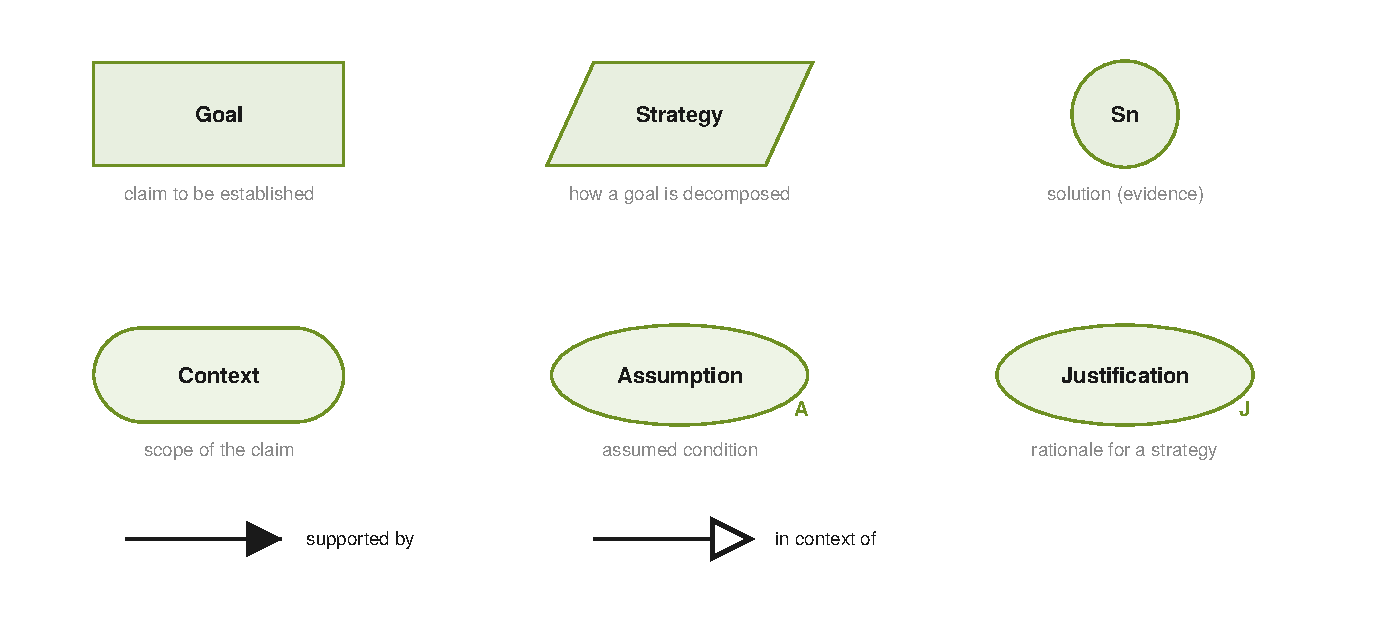
\includegraphics[width=15cm]{gsn_notation}
    \caption{Core element types of the Goal Structuring Notation used in this thesis:
    goal, strategy, solution, context, assumption, and justification, together with
    the supported-by and in-context-of connectors (based on the GSN community standard
    \cite{gsncs2021}).}
    \label{fig:gsn_notation}
\end{figure}
% ---------------------------------------------------------------------------

The \ac{GSN} is adopted here for two reasons. First, its decomposition of a top-level
goal into sub-goals produces the claim hierarchy to which safety performance indicators
are attached in Chapter~\ref{ch:methodology}. Second, a goal that is expressed as a
bare assertion can be turned into a monitorable claim by attaching an indicator to it,
which is the mechanism by which the assurance case is connected to operational data.
The assurance cases of this thesis are modelled in a model-based safety-engineering
environment that supports the construction of \ac{GSN} arguments and their linkage to
other safety artefacts.

\section{Safety Performance Indicators}
\label{sec:fund_spi}

A \ac{SPI} is a metric, supported by evidence, that uses a threshold comparison to
condition a claim within a safety assurance case; it is a metric-threshold pair that
measures a specific aspect of safety \cite{laxman2024}. Three parts therefore make up
every \ac{SPI}, and all three are needed. The first is the metric, a quantity computed
from data, such as a count, a rate, or a physical measurement. The second is the
threshold, a value that separates acceptable from unacceptable, against which the metric
is compared. The third is the claim, the specific statement in the assurance case that
the comparison is taken to support or to challenge. A metric on its own does not
constitute an \ac{SPI}, because the same numerical value can be acceptable in one
operating context and unacceptable in another; only when the metric is paired with a
threshold and tied to a claim does it carry a safety meaning
\cite{laxman2024, koopman2022howsafe}.

Metrics may be quantitative or qualitative. A quantitative metric is a measured or
counted value, for example a rate of events per distance driven, whereas a qualitative
metric records the presence or the completeness of a process step, for example whether
a required review has been carried out. Because context governs acceptability, the
threshold is frequently conditioned on the operating conditions, so that the value
regarded as acceptable in one part of the \ac{ODD} differs from that in another. The
threshold itself has two distinct roles that are developed in
Chapter~\ref{ch:methodology}: a per-event threshold defines what counts as a single
violation, and a rate-level threshold defines how often such violations may occur
before the violation rate itself is anomalous.

The property that matters most for this thesis is whether an indicator is leading or
lagging, according to whether it is observed before or after a loss event. A lagging
\ac{SPI} reports an outcome after the fact; the collision rate, the injury rate, and
the count of automation disengagements are lagging indicators of an \ac{ADS}. A leading
\ac{SPI} observes a condition that precedes a loss event and therefore offers the
opportunity to act before it occurs; the rate at which the time-to-collision falls
below a set value, the rate of activation of automatic emergency braking, and the rate
at which a following gap drops below a safe distance are leading indicators
\cite{koopman2022howsafe}. An effective programme combines both, but only leading
indicators enable a proactive response, which is why their systematic construction is
the central concern of this work.

A concrete example makes the structure explicit. Consider the assurance-case goal that
the vehicle keeps a safe separation from a leading vehicle. A candidate leading \ac{SPI}
for this goal pairs the time-to-collision metric of Section~\ref{sec:fund_metrics} with
a per-event threshold $\theta$ and a rate-level threshold $T$, and conditions the goal
in the form given in Equation~\ref{eq:spi_example}.

\begin{equation}
    \mathrm{count}\!\left(\mathrm{TTC}_{\min} < \theta\right)\ \mathrm{per}\ N\ \mathrm{manoeuvres}\ <\ T
    \label{eq:spi_example}
\end{equation}
\equationentry{Example leading safety performance indicator on time-to-collision}

where $\mathrm{TTC}_{\min}$ is the minimum time-to-collision observed during a
manoeuvre, $\theta$ is the per-event threshold below which the manoeuvre counts as a
violation, $N$ is a fixed number of manoeuvres over which the count is taken, and $T$
is the rate-level threshold. A measured violation rate at or above $T$ challenges the
safe-separation goal and, within an operational safety assurance process, triggers a
review of that part of the assurance case rather than waiting for a collision to be
recorded. The concept, its origin in the aviation safety management systems of the
International Civil Aviation Organization \cite{icao9859}, and its requirement for
automated driving by ANSI/UL~4600 \cite{ul4600} and BSI PAS~1881 \cite{pas1881} are all
introduced here as fundamentals; how a leading \ac{SPI} such as this one is derived
systematically from a claim is the subject of Chapter~\ref{ch:methodology}.

\section{Surrogate Safety Metrics}
\label{sec:fund_metrics}

Because collisions are rare, safety is commonly assessed through surrogate metrics that
quantify how close an interaction comes to a collision, and these metrics supply the
signal component of the indicators derived later. The most established is the
\ac{TTC}, introduced by Hayward, which expresses the time remaining before two road
users on a collision course would collide if their velocities remained unchanged
\cite{hayward1972ttc}. For a following vehicle approaching a leading vehicle along the
same path, the \ac{TTC} is given by Equation~\ref{eq:ttc}.

\begin{equation}
    \mathrm{TTC} = \frac{d_\mathrm{rel}}{v_\mathrm{rel}}, \qquad v_\mathrm{rel} > 0
    \label{eq:ttc}
\end{equation}
\equationentry{Time-to-collision}

where:
\begin{tabbing}
    \hspace{2.2cm} \= \kill
    $d_\mathrm{rel}$ \> relative distance between the two road users in m \\
    $v_\mathrm{rel}$ \> relative closing speed, positive when the gap is closing, in m/s
\end{tabbing}

A related time-based measure is the \ac{PET}, introduced by Allen et al., which
applies to crossing conflicts and measures the time between the moment the first road
user leaves a shared conflict area and the moment the second enters it
\cite{allen1978pet}. A small \ac{PET} indicates that two road users occupied nearly
the same space at nearly the same time. Where a required response is of interest rather
than the time available, the required deceleration to avoid a collision, given in
Equation~\ref{eq:areq}, expresses how hard the vehicle would have to brake, and a value
approaching the physical limit of the vehicle indicates a critical situation.

\begin{equation}
    a_\mathrm{req} = \frac{v_\mathrm{rel}^{2}}{2\,d_\mathrm{rel}}
    \label{eq:areq}
\end{equation}
\equationentry{Required deceleration to avoid a collision}

where:
\begin{tabbing}
    \hspace{2.2cm} \= \kill
    $a_\mathrm{req}$ \> required deceleration in m/s\textsuperscript{2} \\
    $v_\mathrm{rel}$ \> relative closing speed in m/s \\
    $d_\mathrm{rel}$ \> relative distance in m
\end{tabbing}

A formal alternative defines a safe distance from explicit assumptions about
behaviour. The Responsibility-Sensitive Safety model of Shalev-Shwartz et al. defines
the minimum safe longitudinal distance behind a leading vehicle from the response time
and the assumed acceleration and braking capabilities, as given in
Equation~\ref{eq:rss} \cite{shalev2017rss}. A distance below this value denotes a state
that the model regards as unsafe, which makes the model a natural source of a
distance-based threshold.

\begin{equation}
    d_\mathrm{min} = \left[ v_r \rho + \frac{1}{2} a_\mathrm{max}^\mathrm{acc}\,\rho^{2}
    + \frac{\left(v_r + \rho\,a_\mathrm{max}^\mathrm{acc}\right)^{2}}{2\,a_\mathrm{min}^\mathrm{brake}}
    - \frac{v_f^{2}}{2\,a_\mathrm{max}^\mathrm{brake}} \right]_{+}
    \label{eq:rss}
\end{equation}
\equationentry{Responsibility-Sensitive Safety minimum safe longitudinal distance}

where:
\begin{tabbing}
    \hspace{2.2cm} \= \kill
    $v_r,\ v_f$ \> speed of the rear and the front vehicle in m/s \\
    $\rho$ \> response time of the rear vehicle in s \\
    $a_\mathrm{max}^\mathrm{acc}$ \> maximum acceleration during the response time in m/s\textsuperscript{2} \\
    $a_\mathrm{min}^\mathrm{brake}$ \> minimum braking of the rear vehicle in m/s\textsuperscript{2} \\
    $a_\mathrm{max}^\mathrm{brake}$ \> maximum braking of the front vehicle in m/s\textsuperscript{2} \\
    $[\,\cdot\,]_{+}$ \> the positive part, that is $\max(\cdot,0)$
\end{tabbing}

The four measures differ in the conflict geometry for which each is defined and in the
quantity each returns, and Table~\ref{tab:surrogate_metrics} summarises these
differences, since the suitability of a signal for a given conflict is what governs its
selection in Chapter~\ref{ch:methodology}.

% ---------------------------------------------------------------------------
\begin{table}[htbp]
    \centering
    \caption{Surrogate safety metrics used as candidate indicator signals, with the
    conflict geometry for which each is defined, the quantity it returns, and the
    tail in which a critical value lies.}
    \label{tab:surrogate_metrics}
    \small
    \begin{tabular}{@{}p{3.5cm} p{3.3cm} p{3.4cm} p{3.2cm}@{}}
        \toprule
        \textbf{Metric} & \textbf{Conflict geometry} & \textbf{Quantity returned} & \textbf{Critical tail} \\
        \midrule
        Time-to-collision & following, or any conflict with a closing range rate
        & time remaining to contact & lower \\[2pt]
        Post-encroachment time & crossing & time between successive occupancies of a
        shared area & lower \\[2pt]
        Required deceleration & following, and turning conflicts with a defined
        stopping point & braking effort demanded & upper \\[2pt]
        Responsibility-Sensitive Safety distance & longitudinal & minimum admissible
        separation & lower \\
        \bottomrule
    \end{tabular}
\end{table}
% ---------------------------------------------------------------------------

Beyond time- and distance-based measures, model-predictive metrics such as the Model
Predictive Instantaneous Safety Metric of Weng et al. assess safety by predicting the
evolution of a scene under a control model \cite{weng2020mprism}. The geometry of the
two representative conflicts, a following conflict for time-to-collision and required
deceleration and a crossing conflict for post-encroachment time, is shown in
Figure~\ref{fig:metrics_geometry}. The suitability of each metric depends on this
geometry, and a comprehensive survey of criticality metrics and their applicability is
provided by Westhofen et al. \cite{westhofen2023}. This dependence on conflict geometry
is examined further in Chapter~\ref{ch:sota}.

% ---------------------------------------------------------------------------
\begin{figure}[htbp]
    \centering
    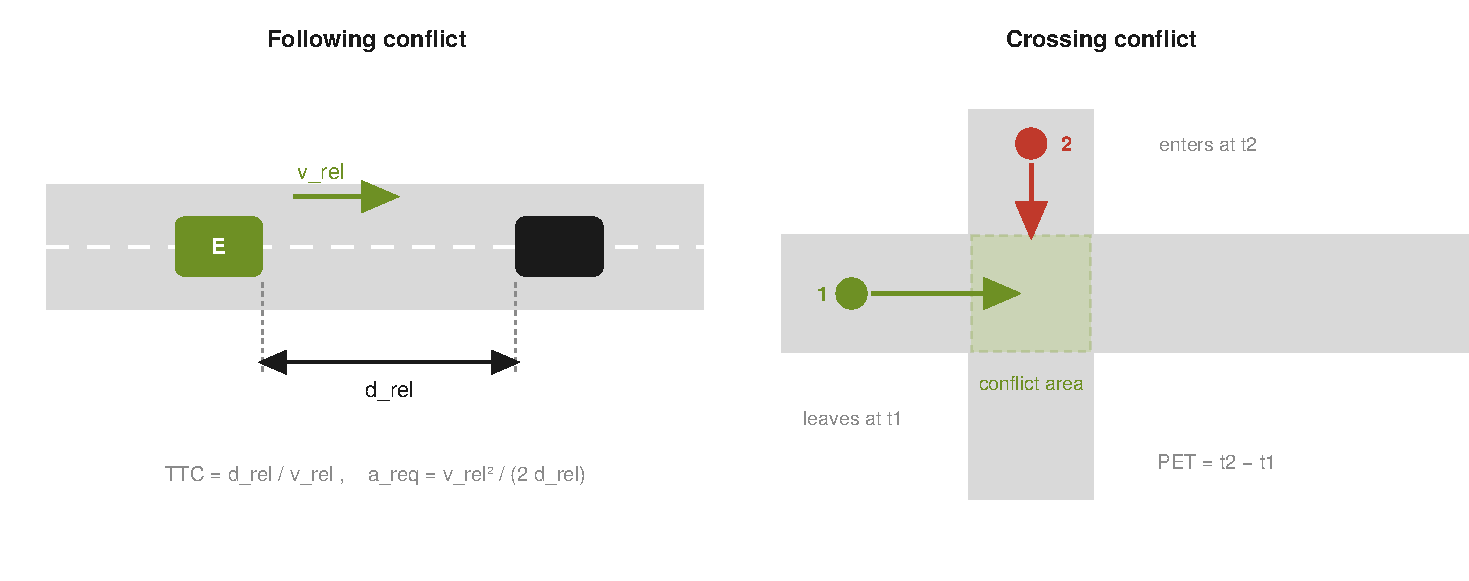
\includegraphics[width=15cm]{surrogate_metrics_geometry}
    \caption{Geometry of the surrogate safety metrics used in this work. Left: a
    following conflict, in which the relative distance and closing speed define the
    time-to-collision and the required deceleration. Right: a crossing conflict, in
    which the post-encroachment time is the interval between the first road user
    leaving and the second entering the shared conflict area.}
    \label{fig:metrics_geometry}
\end{figure}
% ---------------------------------------------------------------------------

\section{Simulation-Based Safety Assessment}
\label{sec:fund_sim}

Because field data on rare safety-critical events is sparse and reporting is
inconsistent, safety-critical behaviour is studied in simulation, where scenarios can
be generated in large numbers and with controlled parameters. CARLA is an open-source
simulator for automated driving research that provides sensor models, traffic
participants, and configurable environmental conditions, together with a programmable
interface for scripting scenarios and logging ground-truth state \cite{dosovitskiy2017carla}.
In this thesis it is used to generate the scenarios from which the derived indicators
are evaluated. The use of ground-truth state has an important consequence for the scope
of the evaluation, which is discussed in Chapter~\ref{ch:methodology}, because signals
that depend on the internal outputs of a perception module cannot be observed when the
ego vehicle is driven by a rule-based agent on ground truth.
\chapter{State of the Art}
\label{ch:sota}

Whereas the fundamentals establish the terminology of safety assurance, safety
argumentation, and safety performance indicators, this chapter reviews the
\textit{current} state of research on their combined use for operational safety
assurance of \ac{ADS}. The review is organised from the general to the specific. It
begins with structured safety argumentation and the shift towards operational
assurance, narrows to \ac{SPI} based safety performance monitoring, then examines the
accident causation and investigation methods that supply the reasoning for deriving
indicators, surveys how mature safety domains transform lagging indicators into
leading ones, reviews the surrogate safety metrics that serve as candidate signals,
and closes with a consolidated statement of the research gap that motivates the
methodology in Chapter~\ref{ch:methodology}. Each section concludes with the aspect
that remains open.

\section{Structured Safety Argumentation for Automated Driving Systems}
\label{sec:sota_argumentation}

Safety assurance cases and the Goal Structuring Notation are introduced in
Section~\ref{sec:fund_gsn}; this section reviews how they are treated in current
research on automated driving. Among the available notations, namely the
Claims-Arguments-Evidence notation, the Structured Assurance Case Metamodel, and the
\ac{GSN}, the \ac{GSN} is the most widely used in safety-critical domains, and its
decomposition of a top-level goal into sub-goals provides the claim hierarchy to
which indicators are attached in this work \cite{kelly2004gsn}.

The assurance case for an \ac{ADS} is valid at the time of its submission to a
certification authority, based on the evidence available during development
\cite{laxman2024}. For automated driving, however, new or contradictory information
can emerge after deployment, revealing emergent system properties, environmental
uncertainties, or divergences in component performance that undermine the validity
of the original argument \cite{laxman2025}. Assurance cases are intended to be living
documents, yet in conventional practice they are treated as static artefacts that
are signed off once \cite{laxman2025}. The central limitation of pure design-time
argumentation is therefore that it cannot, on its own, account for the open and
dynamic operating environment of an \ac{ADS}.

\section{Operational Safety Assurance}
\label{sec:sota_operational}

Operational safety assurance addresses the limitation above by maintaining confidence
in the validity of the assurance case after deployment, using the growing
availability of field data \cite{laxman2024}. Research in this direction is gaining
traction, particularly for runtime model-based assurance cases. Wei et al. argue for
the transition from design-time to runtime assurance-case processes on the basis of
the Structured Assurance Case Metamodel \cite{wei2024access}, and Asaadi et al.
introduce dynamic assurance cases as a pathway to trusted autonomy for systems based
on artificial intelligence and machine learning \cite{asaadi2020dynamic}. Carlan et
al. extend this line of work to a dynamic safety-case management system for frontier
artificial-intelligence systems \cite{carlan2024dynamic}. These approaches establish
that the assurance case is to be treated as a dynamic artefact rather than a fixed
document.

A second line of research improves the rigour of the argument itself so that its
runtime challenges become explicit. Assurance~2.0 retains the structure of
traditional assurance cases but emphasises rigorous evidence assessment and the
active search for defeaters in order to counter confirmation bias
\cite{bloomfield2020assurance2}. Eliminative argumentation provides the underlying
mechanism, in which claims are recursively challenged by doubts, termed defeaters,
and confidence in a claim increases as these defeaters are resolved by additional
argumentation or evidence \cite{goodenough2015ea}. Three types of defeater are
distinguished, namely rebutting, undermining, and undercutting defeaters
\cite{laxman2025}. Diemert et al. build on this notion with incremental assurance, in
which confidence in an eliminative argument is raised by supplying additional
evidence that resolves the recorded defeaters \cite{diemert2023incremental}. Hawkins
and Ryan Conmy complement design-time argumentation with dialectic analysis, which
identifies how an argument may be challenged at runtime and derives corresponding
runtime monitoring requirements in a systematic manner \cite{hawkins2023dialectic}.
The common contribution of these approaches is a structured record of doubt. The open
aspect is that the resolution of many defeaters requires operational data that is
unavailable before deployment.

The integration of field data into this process is the specific concern of the
SafetyDevOps paradigm. The SafeOps approach applies the principles of automation,
feature-driven development, and operational monitoring to the iterative extension of
safety-critical products under ISO~26262 \cite{munk2022safeops}. Building on this,
Laxman et al. propose a cumulative operational safety assurance approach in which risk
assessment, safety measures, requirements, and their validation are built up
iteratively over time together with field data, so that the assurance case is
enhanced continuously rather than fixed at release \cite{laxman2024}. The authors
identify the absence of systematic methods for leveraging runtime vehicle data in a
cumulative manner as a principal research gap \cite{laxman2024}. This position
establishes the process context of the present work, but it does not by itself
specify which quantities are to be monitored.

\section{Safety Performance Indicators}
\label{sec:sota_spi}

Safety performance indicators, defined in Section~\ref{sec:fund_spi}, are the
mechanism by which field data is connected to the claims of an assurance case, and
their use is mandated for automated driving by ANSI/UL~4600 in its Section~16
\cite{ul4600} and by BSI PAS~1881 \cite{pas1881}, with complementary field-monitoring
obligations arising from ISO~26262 \cite{iso26262} and ISO~21448 \cite{iso21448}. The
research question is therefore not whether indicators are required, which the standards
settle, but how a useful set of them is obtained.

The distinction between leading and lagging indicators (Section~\ref{sec:fund_spi}) is
the organising property of the research. Diaz and Woon observe that the lower the level
of the safety-case claim to which an indicator is attached, the more likely it is to be
a leading indicator, because low-level claims are violated earlier than the high-level
outcomes they support \cite{diaz2022drspi}. This relationship between claim depth and
indicator lead time is illustrated in Figure~\ref{fig:spi_spectrum} and is central to
the derivation strategy pursued in this work. ANSI/UL~4600 reflects the same priority,
stating in its guidance that reliance on lagging indicators alone is not acceptable,
yet the standard provides only examples of indicators and leaves their derivation to
the practitioner \cite{ul4600}.

% ---------------------------------------------------------------------------
\begin{figure}[htbp]
    \centering
    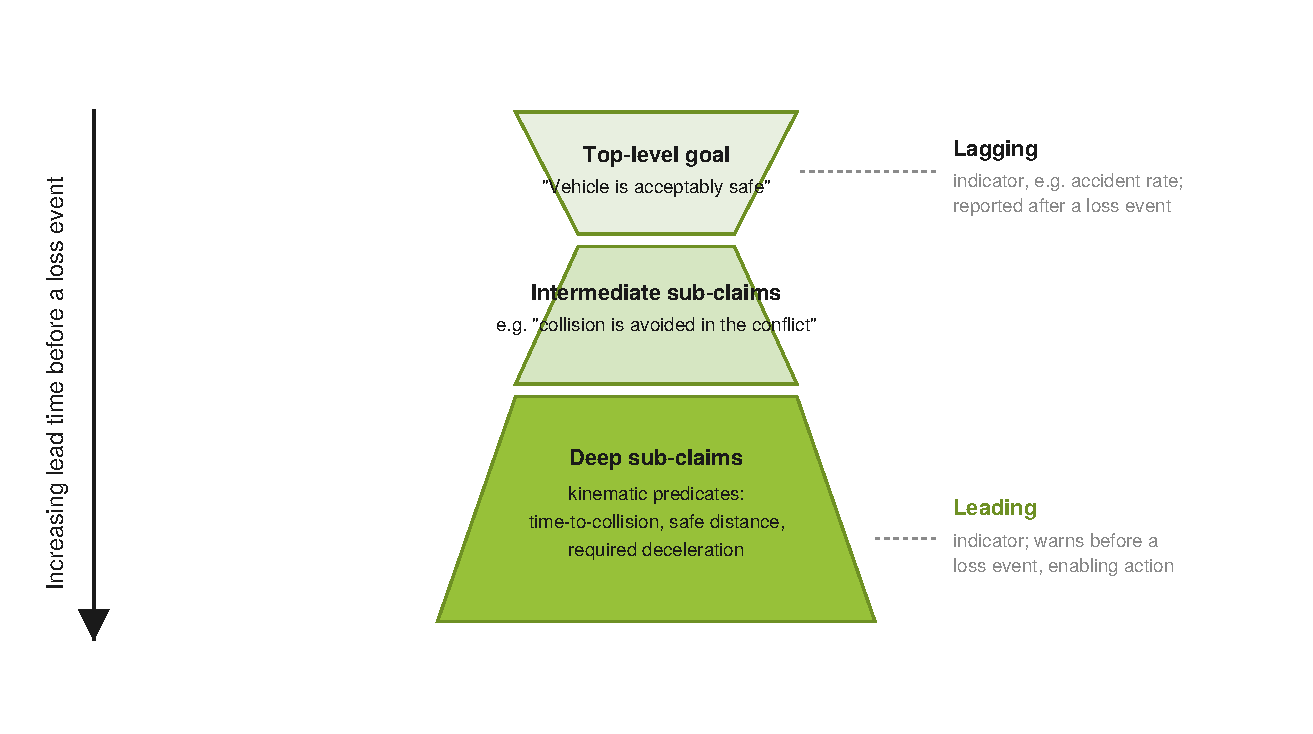
\includegraphics[width=15cm]{spi_leading_lagging_spectrum}
    \caption{Relationship between the depth of a safety-case claim and the leading or
    lagging character of the attached safety performance indicator. Indicators on deep
    sub-claims tend to be leading and provide earlier warning, whereas indicators on
    high-level claims tend to be lagging (based on \cite{diaz2022drspi} and
    \cite{koopman2022howsafe}).}
    \label{fig:spi_spectrum}
\end{figure}
% ---------------------------------------------------------------------------

Several frameworks build on this leading-indicator property. The Dynamic Realtime
\ac{SPI} framework of Diaz and Woon attaches indicators computed at runtime to
sufficiently low safety-case sub-claims, so that a threshold violation signals that
the \ac{ADS} is encountering an untested situation, and assigns each such indicator an
improvement mechanism that adjusts vehicle behaviour to re-establish the validity of
the sub-claim \cite{diaz2022drspi}. Ratiu et al. address a complementary concern,
namely that the rationale by which a chosen set of \acp{SPI} contributes to safety is
often left implicit. They propose an explicit argument pattern for the use of
\acp{SPI}, analyse the defeaters that can undermine confidence in a chosen indicator
set, and introduce meta-indicators that monitor whether the indicators themselves
continue to perform as intended \cite{ratiu2024}. The systematic derivation of
indicators from an assurance case is addressed most directly by Laxman et al., whose
four-step approach represents the uncertainty of assurance-case claims using
Dempster-Shafer theory, propagates this uncertainty to the top goal, resolves claims
through eliminative argumentation, and defines \acp{SPI} for those claims that cannot
be resolved without runtime data \cite{laxman2025}. To the knowledge reported in that
work, no standard or otherwise widely used systematic approach for specifying
\acp{SPI} exists \cite{laxman2025}. The open aspect is that the derivation of a
\emph{leading} indicator from a \emph{lagging} one is not itself formalised, and the
reasoning that justifies why a given signal predicts a given loss event is drawn from the
accident investigation literature reviewed next.

\section{Accident Causation Models and Investigation Methods}
\label{sec:sota_causation}

The derivation of a leading indicator from a loss event rests on a model of how that
loss event is caused, and such models originate in accident investigation, which is
inherently a reactive activity performed after a loss. Three families of causation
model are relevant. The first is the sequential, component-failure family, of which
Fault Tree Analysis is the archetype. Fault Tree Analysis is a deductive, top-down
method that starts from an undesired top event and uses Boolean logic gates,
principally AND and OR, to decompose it into intermediate events and finally basic
events with associated failure data \cite{ericson1999,nasaftahandbook}. It is
codified in IEC~61025 \cite{iec61025} and, for automotive systems, recommended by
ISO~26262 for the higher automotive safety integrity levels \cite{iso26262}. The
top-down AND and OR decomposition supplies the structural skeleton for deriving
indicators, because a loss event treated as a top event decomposes into the
subsystem-level causes and observable signals that precede it. The recognised
limitation of classical Fault Tree Analysis is its assumption of discrete,
independent component failures, which does not capture the functional insufficiencies
of a machine-learning perception stack, where a component operates as specified yet
the specification itself is inadequate \cite{ruijters2015}. The structure is shown
schematically in Figure~\ref{fig:fault_tree}: Boolean reduction of the tree yields
minimal cut sets, the smallest combinations of basic events sufficient to cause the
top event, and these map directly onto the candidate signal sets from which leading
indicators are drawn.

% ---------------------------------------------------------------------------
\begin{figure}[htbp]
    \centering
    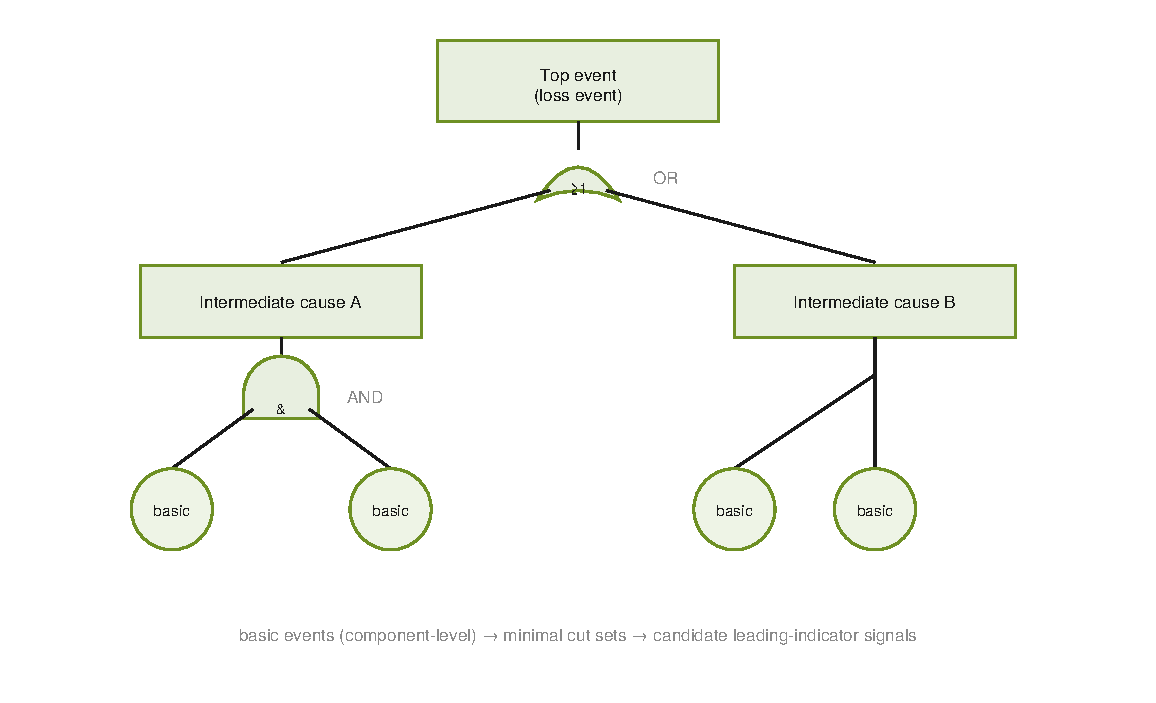
\includegraphics[width=13cm]{fault_tree_example}
    \caption{Deductive top-down structure of a fault tree: an undesired top event is
    decomposed through OR and AND gates into intermediate events and basic events
    (recreated, based on the fault-tree method of IEC~61025 \cite{iec61025}).}
    \label{fig:fault_tree}
\end{figure}
% ---------------------------------------------------------------------------

The second family is the epidemiological, barrier-based model. Reason's organisational
accident model distinguishes active failures from latent conditions and holds that an
accident occurs when weaknesses in successive defensive layers momentarily align
\cite{reason1990,reason2000}. The bowtie method operationalises this view by combining
a fault tree of threats leading to a central loss event with an event tree of
consequences, and by making the preventive and mitigating barriers explicit
\cite{ccps2018bowties}. The health of each barrier can then be monitored by a
dedicated leading indicator, which is the conceptual bridge from a causation model to
an \ac{SPI}. Application of the bowtie method to road-traffic and cooperative-driving
safety exists but remains uncommon \cite{ehlers2017}, and a comprehensive treatment
for a full \ac{ADS} safety case is not established. The relationship between the two
views is shown in Figure~\ref{fig:bowtie}, where the bowtie places the fault tree and
the event tree on either side of a central loss event, with the barriers whose health
a leading indicator monitors sitting on the preventive side.

% ---------------------------------------------------------------------------
\begin{figure}[htbp]
    \centering
    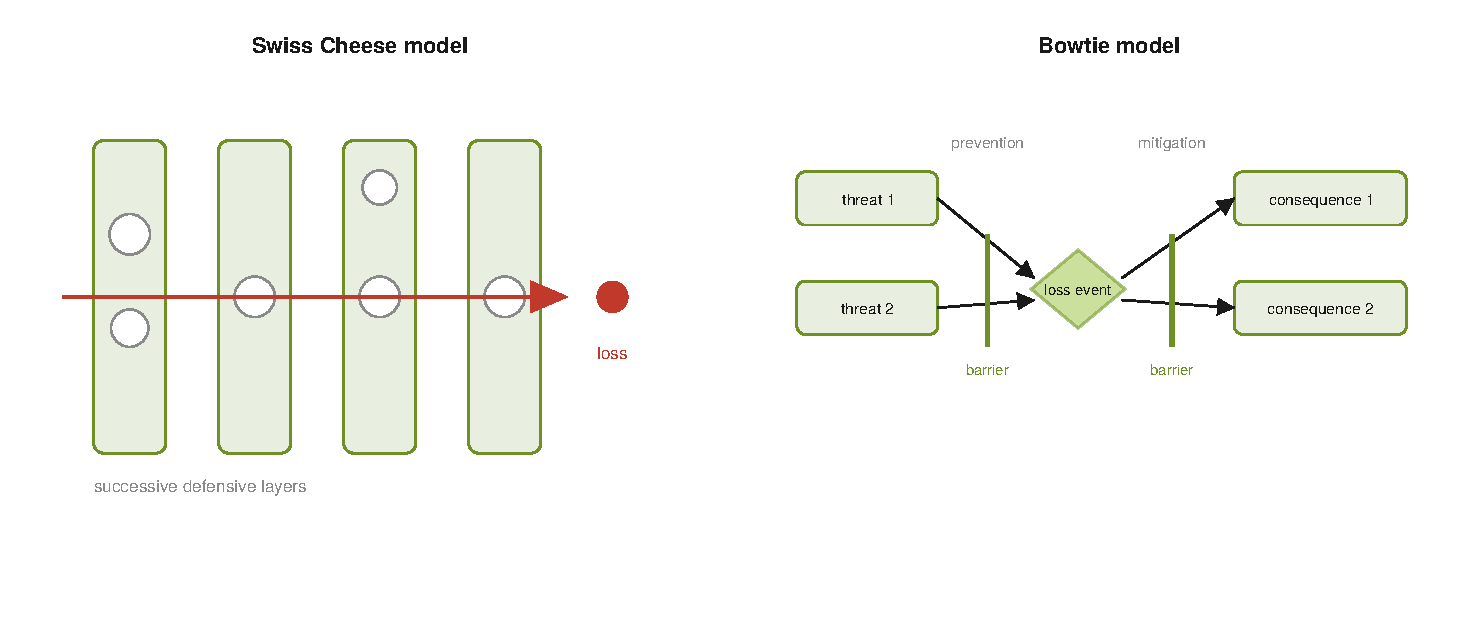
\includegraphics[width=15cm]{swiss_cheese_bowtie}
    \caption{Barrier-based accident model. Left: the Swiss Cheese view, in which a loss
    event occurs when weaknesses in successive defensive layers align. Right: the
    bowtie, combining a fault tree of threats and an event tree of consequences around
    a central loss event, with preventive and mitigating barriers made explicit
    (recreated, based on \cite{reason2000} and \cite{ccps2018bowties}).}
    \label{fig:bowtie}
\end{figure}
% ---------------------------------------------------------------------------

The third family is the systemic, control-theoretic model. The Systems-Theoretic
Accident Model and Processes reframes safety as the enforcement of constraints within
a hierarchical control structure rather than as a chain of component failures
\cite{leveson2011}. Its hazard-analysis technique, System-Theoretic Process Analysis,
identifies unsafe control actions and their causal scenarios \cite{stpahandbook}, and
its investigation counterpart, Causal Analysis based on System Theory, reconstructs
the control-structure failures behind an accident \cite{casthandbook}. Unsafe control
actions are candidate leading indicators, and the approach captures the non-failure,
functional-insufficiency hazards that Fault Tree Analysis misses under the safety of
the intended functionality \cite{iso21448}. The open aspect is that System-Theoretic
Process Analysis and Causal Analysis based on System Theory are qualitative and do
not natively produce thresholds or continuously monitored indicators
\cite{khastgir2021}. The hierarchical control view is shown in
Figure~\ref{fig:stamp}, in which each control action and feedback path is a place where
an unsafe control action, and hence a candidate leading indicator, can be located.

% ---------------------------------------------------------------------------
\begin{figure}[htbp]
    \centering
    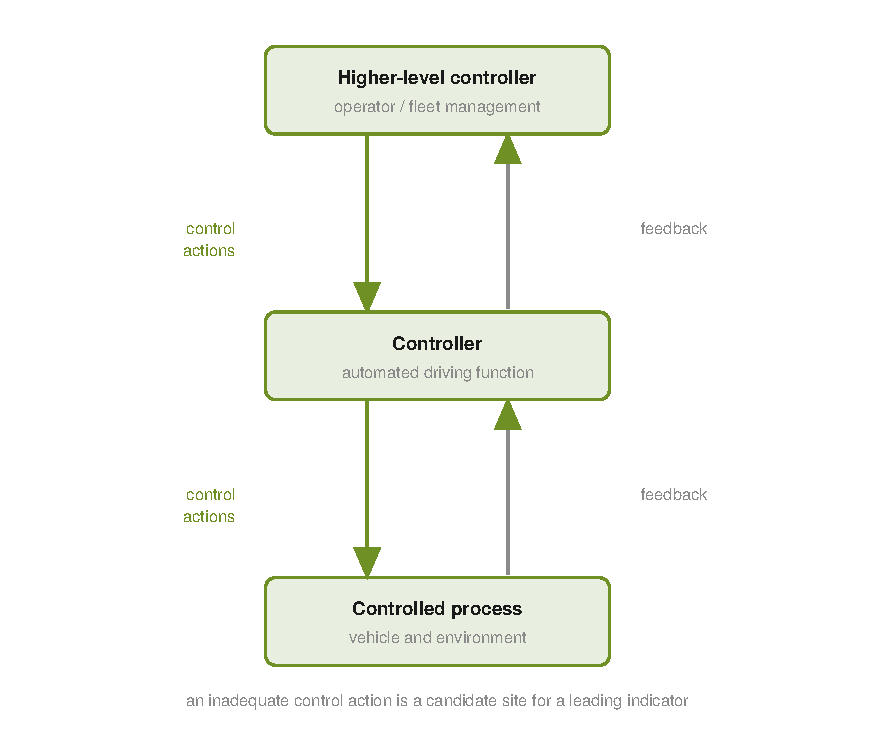
\includegraphics[width=11cm]{stamp_control_structure}
    \caption{Hierarchical control structure of the Systems-Theoretic Accident Model and
    Processes. Safety is treated as the enforcement of constraints through control
    actions, with feedback informing each controller; inadequate control actions are
    the candidate sites for leading indicators (recreated, based on \cite{leveson2011}).}
    \label{fig:stamp}
\end{figure}
% ---------------------------------------------------------------------------

A distinct contribution comes from formal incident analysis. Why-Because Analysis
constructs a directed acyclic causal graph in which a factor is admitted as a cause
only if it passes a counterfactual test, that is, whether the effect would still have
occurred had the factor been absent \cite{ladkin1998}. This counterfactual test is
functionally identical to the prevention test used in the methodology of this work to
identify a proximate cause, and it therefore provides a formal, citable grounding for
that step. The open aspect common to all of these methods is that they are
retrospective and manual, applied to a single incident after the fact, and none has
been operationalised to generate forward-looking, continuously monitored indicators
for an \ac{ADS}.

\section{From Reactive Investigation to Proactive Monitoring}
\label{sec:sota_reactive_proactive}

The methods of Section~\ref{sec:sota_causation} are reactive, since they analyse a loss
that has already occurred, and the value of an \ac{SPI} lies in converting their
insight into a proactive signal that acts before a loss. Precursor analysis supplies the
theory for this conversion. It treats near-misses and off-nominal events as truncated
accident sequences that carry predictive information about rare, high-consequence
events, and uses Bayesian methods to update accident-likelihood estimates from
abundant low-severity data \cite{bieryi1995,saleh2013}. A leading indicator is, in
these terms, a formalised precursor, and precursor-estimation theory offers a
principled route to calibrating indicator thresholds from sparse loss data. The
associated caution is equally important. The fixed-ratio safety pyramid of Heinrich,
which assumes a stable numerical relationship between minor and major events
\cite{heinrich1931}, is contested by later evidence. Yorio and Moore, analysing 27,446
mining establishments over the period 2000 to 2012, find no significant difference in
the probability of a subsequent fatal event between establishments with few and with
zero lost or restricted days \cite{yoriomoore2018}. The quantitative link between a
precursor and a loss event must therefore be validated empirically rather than assumed.

Aviation demonstrates the reactive-to-proactive transition in mature form. Its safety
management system institutionalises a continuous loop that monitors indicators,
detects deviations, manages risk, and verifies the result \cite{icao9859}, and Flight
Operational Quality Assurance mines routine flight data for exceedances that act as
precursors before an accident occurs. This is the same lagging-to-leading
transformation that the present work systematises for automated driving, and it is
widely regarded as the origin of the \ac{SPI} concept later adopted by ANSI/UL~4600.
Within automated driving, the equivalent sentinel signal is the activation of
Autonomous Emergency Braking, a last-resort intervention triggered when normal control
has failed to preserve an adequate margin, typically parameterised by time-to-collision
\cite{eNCAP_aeb}. A rising activation rate is an early-warning precursor of collision
risk. The published treatment of Autonomous Emergency Braking is, however, oriented
towards component testing under rating protocols rather than towards a monitored fleet
indicator with a calibrated threshold feeding a safety case.

The lagging indicators of automated driving are documented in crash and disengagement
data. Analyses of the California disengagement and collision reports report, for
example, an average of one accident per 178 disengagements up to July 2017
\cite{favaro2018}, and the reporting mandated by the United States National Highway
Traffic Safety Administration provides a growing but incomplete record of automation-
involved crashes \cite{nhtsa_sgo}. The investigation of the Tesla Autopilot design by
that agency reviewed 956 crashes in which the system was alleged to have been engaged,
analysed 467 after exclusions, identified at least 13 involving one or more
fatalities, and concluded that the design contributed to foreseeable misuse and
avoidable crashes \cite{nhtsa_ea22002}. The same investigation records that only about
18 per cent of police-reported crashes involve an airbag deployment and that the
manufacturer largely receives data only for such crashes, which exposes the sparsity
and reporting bias of field lagging data \cite{nhtsa_ea22002}. This limitation is the
direct justification for generating leading indicators in simulation, as pursued in
this work, rather than relying on sparse field data.

\section{Deriving Leading Indicators from Lagging Indicators}
\label{sec:sota_derivation}

Mature safety domains beyond automated driving have converged on the practice of
pairing leading and lagging indicators, which frames the specific gap this work
addresses. In process safety, the guidance of the Center for Chemical Process Safety
and the recommended practice API~RP~754 define a tiered structure in which the higher
tiers are lagging outcome events and the lower tiers are leading indicators of barrier
and system performance, derived from the weaknesses of the barriers in a Swiss Cheese
or bowtie model \cite{ccps2018metrics,apirp754}. The step-by-step guide HSG254 of the
United Kingdom Health and Safety Executive adds the concept of dual assurance, pairing
a leading and a lagging indicator for each critical risk-control system
\cite{hse2006hsg254}. Across these domains the distinction is consistent, with lagging
indicators being retrospective, few, and severe, and leading indicators being
forward-looking and numerous.

Table~\ref{tab:crossdomain} sets the four domains side by side, which makes the common
structure and the common omission visible in one view.

% ---------------------------------------------------------------------------
\begin{table}[htbp]
    \centering
    \caption{Pairing of leading and lagging indicators across mature safety domains,
    showing the source of the leading indicator in each domain and whether a
    reproducible derivation procedure is published.}
    \label{tab:crossdomain}
    \small
    \begin{tabular}{@{}p{2.7cm} p{3.1cm} p{4.0cm} p{3.4cm}@{}}
        \toprule
        \textbf{Domain} & \textbf{Lagging indicator} & \textbf{Source of the leading indicator} & \textbf{Derivation procedure} \\
        \midrule
        Process safety \cite{ccps2018metrics,apirp754} & tiered loss-of-containment
        events & barrier weaknesses in a bowtie model & tiered structure given;
        derivation by expert judgement \\[2pt]
        Occupational safety \cite{hse2006hsg254} & lost-time and reportable
        incidents & risk-control systems, paired by dual assurance & pairing
        prescribed; derivation by expert judgement \\[2pt]
        Aviation \cite{icao9859} & accidents and serious incidents & routine
        flight-data exceedances & continuous monitoring institutionalised;
        derivation by expert judgement \\[2pt]
        Automated driving \cite{ul4600,ratiu2024} & collisions and
        disengagements & safety-case claims and surrogate metrics & none published;
        stated as an open gap \\
        \bottomrule
    \end{tabular}
\end{table}
% ---------------------------------------------------------------------------

The consistent shortfall is that the derivation itself is driven by expert judgement
rather than by a reproducible procedure. In every case a practitioner identifies
barriers from a causation model and then defines indicators of barrier health, and no
domain publishes a validated, step-by-step method that takes a specific lagging
indicator and produces calibrated leading indicators with explicit observability and
independence checks. For automated driving the gap is stated directly in the
literature. Ratiu et al. observe that there is no systematic discussion of the
challenges of deploying \acp{SPI} and frame their own contribution as only an initial
step towards a systematic framework \cite{ratiu2024}, and Diaz and Woon classify each
indicator as leading or lagging case by case rather than deriving them systematically
\cite{diaz2022drspi}. This absence of a reproducible derivation procedure is the
precise gap that the methodology of this work fills.

\section{Safety Metrics as Candidate Indicators}
\label{sec:sota_metrics}

The metric component of an \ac{SPI} is drawn from the body of surrogate safety
metrics defined in Section~\ref{sec:fund_metrics}, and the suitability of a metric
determines the quality of the resulting indicator. Fraade-Blanar et al. provide a
framework for measuring automated-vehicle safety that organises these measures along a
leading-to-lagging axis and catalogues their respective strengths and weaknesses
\cite{fraadeblanar2018}, and Westhofen et al. survey the wider landscape of criticality
metrics and analyse their suitability for different conflict types \cite{westhofen2023}.
The value of these metrics as established, pre-validated loss predictors means that the
derivation of this work can treat the signals as known and claim novelty in the
derivation procedure rather than in the predictive power of each signal.

\section{Conflicts in the Target Manoeuvre}
\label{sec:sota_conflicts}

The manoeuvre evaluated in this work, an unprotected left turn, folds together three
conflicts of different character, and the literature treats each with different metrics
and reports different limitations for each. Reviewing them separately establishes why a
single derivation method must be tested against all three rather than assumed to
transfer.

The first is the oncoming-vehicle conflict, a longitudinal left-turn-across-path
interaction. Studies of automated vehicles at unsignalised intersections report that
this conflict is among the most demanding, because the decision window is short and the
turn crosses the path of oncoming traffic \cite{leftturn_unsignalized}. Field testing
of driver-assistance systems in naturalistic left-turn-across-path conditions reports
that automatic emergency braking failed to activate braking early enough even when the
detection criteria were technically met, with decision windows on the order of three
seconds \cite{leftturn_field2025}. This indicates that a purely detection-based
indicator offers poor lead-time adequacy in this conflict.

The second is the pedestrian-crossing conflict, a crossing interaction for which
post-encroachment time rather than pure time-to-collision is the natural surrogate
measure \cite{allen1978pet}. Pedestrian protection is assessed in rating protocols
through dedicated automatic-emergency-braking pedestrian tests \cite{eNCAP_aeb}, yet
studies of such systems at intersections show that occlusion, in which the pedestrian
is hidden until late, sharply reduces the available response time and the achievable
avoidance rate \cite{ped_aeb_occluded}. The adequacy of a crossing indicator therefore
depends strongly on when the crossing road user first becomes observable, which differs
in character from the oncoming conflict.

The third is the rear-end, or following, conflict, in which the ego vehicle must
maintain a safe separation from a vehicle behind it while it decelerates for the turn.
The established surrogate measures here are time headway and the Responsibility-Sensitive
Safety safe distance \cite{shalev2017rss}, and recent work estimates rear-end collision
risk for automated vehicles in mixed traffic from real-world perception data
\cite{rearend_av2025}. The controlling quantity is the follower's ability to respond to
the ego vehicle's deceleration, which is again a different mechanism from the other two
conflicts.

Taken together, the three conflicts have distinct geometries and distinct
controlling quantities, so the adequacy of a given metric as a leading indicator is
conflict-dependent. This is the direct motivation for deriving and evaluating indicators
separately by conflict actor in Chapter~\ref{ch:methodology} and
Chapter~\ref{ch:results}, rather than assuming one indicator serves the whole manoeuvre.

\section{Research Gap}
\label{sec:sota_gap}

The reviewed literature supports a single, focused research gap. Structured
argumentation and operational-assurance approaches
(Section~\ref{sec:sota_argumentation}, Section~\ref{sec:sota_operational}) establish
that an assurance case must be maintained with field data through a SafetyDevOps
process. The \ac{SPI} literature (Section~\ref{sec:sota_spi}) establishes the
metric-threshold definition of an indicator, the value of leading indicators on deep
sub-claims, and a first systematic method for identifying which claims require
indicators. The accident-causation and cross-domain literature
(Section~\ref{sec:sota_causation} to Section~\ref{sec:sota_derivation}) supplies the
reasoning components, namely fault-tree decomposition, the counterfactual prevention
test, precursor theory, and barrier-health monitoring, but no domain integrates them
into a reproducible procedure. The metric literature (Section~\ref{sec:sota_metrics})
provides candidate signals and evidence that their adequacy depends on the conflict
type.

Three deficiencies remain. First, no reproducible method derives a set of leading
\acp{SPI} from a lagging \ac{SPI} for an \ac{ADS}; the derivation is left to expert
judgement across every domain, and the gap is stated explicitly for automated driving
\cite{ratiu2024,ul4600}. Second, indicators derived from an assurance case are, to the
extent reported, not evaluated quantitatively against simulation data, so their
ability to detect a developing violation early enough to be actionable, as distinct
from merely detecting that a violation has occurred, is not demonstrated. Third, the
sparsity and reporting bias of field lagging data \cite{favaro2018,nhtsa_ea22002} mean
that the quantitative link between a precursor and a loss event, which the Heinrich critique
shows must not be assumed \cite{yoriomoore2018}, has not been validated for the
relevant conflicts.

This thesis addresses these deficiencies with a systematic causal-chain derivation
method that takes a lagging \ac{SPI}, identifies its proximate cause through a
counterfactual prevention test, decomposes it with fault-tree gate logic to the
subsystem level, extracts the earliest observable signals, checks their observability
and independence, calibrates signal-level and rate-level thresholds, and attaches the
resulting leading \acp{SPI} to a \ac{GSN} safety case modelled in a \ac{GSN} modelling tool.
The indicators are evaluated from simulation data generated in the CARLA simulator
\cite{dosovitskiy2017carla} with an explicit distinction between detection and
lead-time adequacy, separated by conflict actor. The continuous assurance loop within
which the derived indicators operate is summarised in
Figure~\ref{fig:assurance_loop} and frames the methodology that follows.

% ---------------------------------------------------------------------------
\begin{figure}[htbp]
    \centering
    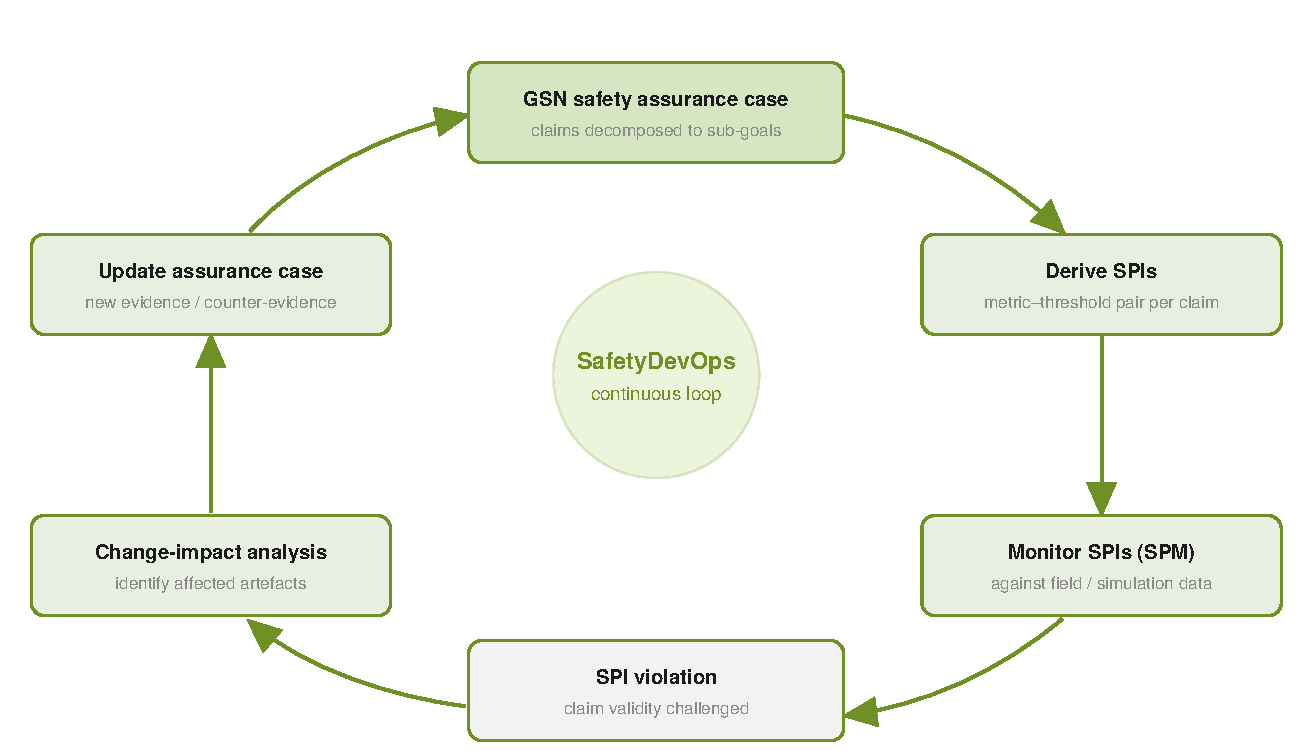
\includegraphics[width=15cm]{spi_assurance_loop}
    \caption{Continuous operational safety assurance loop. Safety performance
    indicators derived from the claims of the assurance case are monitored against
    field or simulation data; a threshold violation triggers a change-impact analysis
    and an update of the assurance case within a SafetyDevOps process (based on
    \cite{laxman2024} and \cite{laxman2025}).}
    \label{fig:assurance_loop}
\end{figure}
% ---------------------------------------------------------------------------
\chapter[Causal Chain Derivation Method]{Method for Causal Chain Derivation of Safety Performance Indicators}
\label{ch:methodology}

This chapter presents the core contribution of the thesis, a systematic Causal Chain
Derivation Method (CCDM) that produces calibrated leading safety performance indicators
from lagging ones and attaches them to a \ac{GSN} safety case. As established in
Chapter~\ref{ch:sota}, the reasoning components already exist in separate literatures
but are not integrated into a reproducible procedure. The method combines three of
them, namely the top-down decomposition of Fault Tree Analysis \cite{iec61025}, the
counterfactual prevention test of Why-Because Analysis \cite{ladkin1998}, and
threshold calibration grounded in precursor-estimation theory \cite{bieryi1995}. The
derived indicators are modelled in a \ac{GSN} modelling tool and evaluated on
simulation data generated in the CARLA simulator \cite{dosovitskiy2017carla}. The chapter first gives
an overview of the seven steps, then describes each step, presents worked examples,
and closes with the properties of the method that carry over into its instantiation
in Chapter~\ref{ch:experiment}.

\section{Overview of the Causal Chain Derivation Method}
\label{sec:method_overview}

The method is defined to be use-case-agnostic, so that it applies without change to a
left-turn, construction-zone, or pedestrian-crossing use case, or to any future one.
It consists of a preparatory step and seven derivation steps, of which
Steps~2 to~7 form a loop executed once for every lagging indicator in the register
built in Step~1. The complete sequence is shown in
Figure~\ref{fig:derivation_flow}. The method is architecture-independent in its
reasoning, because the subsystem decomposition in Step~3 names the functions that any
driving system must perform rather than the components that a particular
implementation contains. Architecture dependence enters only at Step~4, where a
required signal may or may not be exposed by a given implementation, and this
distinction gives rise to the two indicator tiers described in
Section~\ref{sec:method_signal}.

% ---------------------------------------------------------------------------
\begin{figure}[htbp]
    \centering
    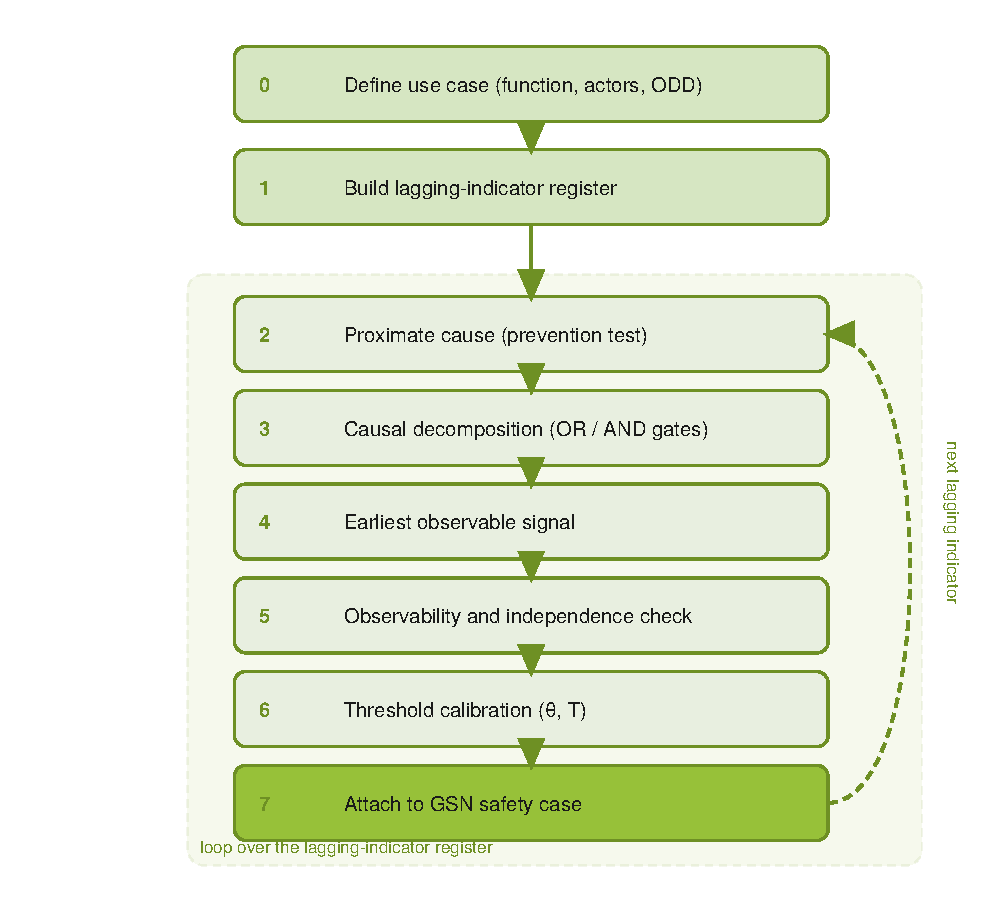
\includegraphics[width=13cm]{spi_derivation_flow}
    \caption{The seven-step causal-chain derivation method. Steps~2 to~7 are executed
    once for each lagging safety performance indicator in the register produced by
    Step~1, and the loop terminates when the register is exhausted.}
    \label{fig:derivation_flow}
\end{figure}
% ---------------------------------------------------------------------------

\section{Use Case and Lagging-Indicator Register}
\label{sec:method_register}

The preparatory step, Step~0, defines the use case in terms of the function the system
performs, the actors present, and the operational design domain. Step~1 then builds
the lagging-indicator register by listing every loss event for the use case as a
lagging \ac{SPI}, each with a single loss-event type and a single unit of measurement.
This register is the set over which the derivation loop iterates. Candidate loss events
are drawn from a catalogue of twelve families, ranging from collision and contact events,
through near-miss and last-resort response events, to control-handover and operating-
domain violations. Near-miss and last-resort response events are the preferred
starting point, because they occur more frequently than collisions yet carry the same
causal information, which mirrors the precursor rationale of
Section~\ref{sec:sota_reactive_proactive}. A selection rule governs the register: each
lagging indicator must resolve to exactly one proximate cause in Step~2, and a
candidate that resolves to several unrelated causes is defined too broadly and is
split before proceeding.

\section{Proximate Cause by the Prevention Test}
\label{sec:method_proximate}

Step~2 identifies the proximate cause of each lagging indicator by applying the
prevention test, which asks whether the loss event would have been prevented if one
condition had been corrected at the last possible moment. This test is the
counterfactual test of Why-Because Analysis applied prospectively
\cite{ladkin1998}. The answer is expressed as a functional impossibility in passive
form, of the type that the system could not perform a required action, and exactly one
proximate cause is admitted per lagging indicator. The boundary between a proximate
and an intermediate cause is set by whether a response window remained after the
failure. If a detection failure left no time for any response, the detection failure
is the proximate cause, whereas if a response window remained and was not used, the
detection failure is an intermediate cause and the resulting avoidance failure is the
proximate cause.

\section{Causal Decomposition with Gate Logic}
\label{sec:method_decomposition}

Step~3 decomposes the proximate cause into intermediate causes using the gate logic of
Fault Tree Analysis \cite{iec61025}. An OR gate applies when any one cause is
sufficient on its own, which requires a separate leading indicator for each branch and
is the common case for perception and planning failures. An AND gate applies when the
causes must co-occur because redundancy is present, in which case a single shared
indicator can suffice. The gate for a pair of candidate causes is determined by asking
whether either cause alone can produce the proximate cause without the other. The
decomposition terminates when each cause maps to exactly one functional subsystem,
namely perception, prediction, planning, control, or operating-domain monitoring, and
is describable by a quantity that any implementation of that subsystem would produce.
Deeper decomposition is deliberately avoided, because it reaches algorithm-specific or
sensor-specific detail and breaks the implementation-agnostic character of the method.
A supplementary System-Theoretic Process Analysis cross-check is recommended for
control-loop and non-failure hazards that Fault Tree Analysis does not capture under
the safety of the intended functionality \cite{iso21448,stpahandbook}.

The use of gate logic requires reconciliation with the criticism of Fault Tree Analysis
made in Chapter~\ref{ch:sota}, namely that binary component-failure logic does not
represent the continuous, non-failure insufficiencies characteristic of a
machine-learning perception stack. The reconciliation rests on what the gates are
applied to. The decomposition does not enumerate component failure states; it partitions
a proximate cause into functional causes, each of which states that a required function
was not delivered adequately, and adequacy is fixed by the threshold calibrated in
Step~6 rather than by a binary health state. A gate therefore records which functional
shortfalls are jointly or severally sufficient to produce the proximate cause, while the
continuous quantity is carried by the signal and its threshold rather than by the gate.
This preserves the deductive structure that makes the derivation reproducible and places
the continuity where it belongs. One limitation remains and is stated rather than
concealed: a cause arising only from the interaction of two functions, neither of which
is individually inadequate, is not expressible in this logic, and the System-Theoretic
Process Analysis cross-check is the intended remedy for that class of cause.

\section{Observable Signal and Observability Check}
\label{sec:method_signal}

Step~4 names, for each intermediate cause, the earliest measurable quantity with units
that tracks the development of that cause before it fully manifests, together with the
lead time by which it does so. Step~5 then subjects each candidate signal to two tests
that both must pass. The first is computability, meaning that the signal can be
computed at runtime or from available logged data at a sufficient frequency. The
second is independence, meaning that the source of the signal is not the subsystem
being monitored, since a degraded subsystem that reports on itself would appear
healthy at exactly the moment monitoring is required. A signal that fails either test
is unusable regardless of how well it correlates with the loss event, and the requirement to
state signal provenance explicitly is claimed as a contribution, because published
indicator sets rarely record it.

The independence claimed for the behavioural tier requires one qualification, because it
governs how the results of this work transfer to a deployed system. In the simulation
environment of Section~\ref{sec:method_carla} the kinematic quantities are read from
ground truth, which is external to the vehicle software, so a behavioural-tier indicator
is independent of the driving function in the strict sense. In a deployed system no
ground truth exists, and the same quantities are estimated on board by perception and
localisation. A degradation of that estimation chain corrupts the indicator and the
driving function together, so the independence that holds by construction in simulation
becomes an assumption that must be argued separately in deployment, for example by
deriving the indicator from a sensing path not shared with the function it monitors. The
behavioural tier is independent of the planning and control functions it monitors in
both settings, but independent of the perception function only in simulation, and the
results reported for that tier are to be read under this restriction.

The independence requirement partitions the derivable indicators into two tiers,
summarised in Table~\ref{tab:tiers}. Behavioural-tier indicators are computed purely
from vehicle kinematics and scene state and are portable across any architecture,
including an opaque end-to-end network or a human driver. Architectural-tier indicators
require a signal exposed from inside a subsystem and therefore presuppose a modular
pipeline. The trade-off is explicit: behavioural-tier indicators buy portability but
give lower diagnostic resolution, since they reveal that a margin is eroding rather
than which subsystem caused it, and they typically provide shorter lead time, since
internal degradation usually precedes its kinematic consequence.

% ---------------------------------------------------------------------------
\begin{table}[htbp]
    \centering
    \caption{The two indicator tiers produced by the observability and independence
    check of Step~5.}
    \label{tab:tiers}
    \begin{tabular}{l l l}
        \toprule
        \textbf{Property} & \textbf{Behavioural tier} & \textbf{Architectural tier} \\
        \midrule
        Signal source     & vehicle kinematics, scene state & internal subsystem output \\
        Examples          & time-to-collision, closing speed, & detection confidence, \\
                          & required deceleration, PET & time-of-first-detection \\
        Architecture      & portable across any design & modular pipeline required \\
        Diagnostic resolution & margin erosion only & subsystem attribution \\
        Typical lead time & shorter & longer \\
        \bottomrule
    \end{tabular}
\end{table}
% ---------------------------------------------------------------------------

% =============================================================================
% DROP-IN REPLACEMENT for Section 4.6 of Chapter 4 (Method).
% Paste this in place of the existing Section 4.6. It carries the label
% sec:method_thresholds, which Chapters 5, 6 and 7 reference.
% Addresses the fix list: ALARP, GAMAB and MEM named as not applied; T defined
% as the exact one-sided binomial limit at alpha = 0.01 from Campaigns 2 and 3;
% the percentile example corrected to the 10th and 95th.
% =============================================================================

\section{The Metric Threshold and the SPI Threshold}
\label{sec:method_thresholds}

Steps~1 to~5 produce a signal and a source. A signal alone is not yet an
indicator: a quantity becomes a safety performance indicator only once a
threshold decides when its value is to be treated as a violation, and a second
threshold decides when the frequency of such violations is to be treated as a
departure from the argued behaviour. Step~6 sets both, and the general form of an
SPI used throughout this work is given in Equation~(\ref{eq:method_spiform}).

\begin{equation}
    \left\{
        \begin{array}{c}
            \text{No. of times the metric crosses } \theta
            \text{ in the unsafe direction} \\
            \text{per 100k manoeuvres, km or h driven}
        \end{array}
    \right\} < T
    \label{eq:method_spiform}
\end{equation}
\equationentry{General form of a safety performance indicator}

\textbf{Variable key:} $\theta$, metric threshold, in the unit of the metric; T,
SPI threshold, as a count per exposure unit.

The two thresholds answer different questions and are set by different means.
The metric threshold decides a single run and is calibrated from observed
behaviour; the SPI threshold bounds the violation count of a population of runs
and is set statistically. Neither is a risk-acceptance criterion.

\subsection{Setting the Metric Threshold}
\label{sec:method_metricthreshold}

Five ways of setting a metric threshold were considered before the method fixed
on one, and the choice is argued here rather than assumed, because it determines
whether the later evaluation is circular.
Table~\ref{tab:threshold_methods} compares the five by the data and the
assumptions each requires. The comparison is qualitative: no numerical benchmark
between the five was run, and none is implied.

% ---------------------------------------------------------------------------
% Copied verbatim from tables.tex
\begin{table}[htbp]
\centering
\caption{Options for the metric threshold. Five ways to set the metric threshold $\theta$ compared by the data and assumptions they require.}
\label{tab:threshold_methods}
\footnotesize
\setlength{\tabcolsep}{4pt}
\begin{tabular}{@{}>{\raggedright\arraybackslash}p{2.8cm}>{\raggedright\arraybackslash}p{2.1cm}>{\raggedright\arraybackslash}p{3.8cm}>{\raggedright\arraybackslash}p{3.4cm}>{\raggedright\arraybackslash}p{2.3cm}@{}}
\toprule
{\bfseries Method} & {\bfseries Needs collision labels} & {\bfseries Main assumption} & {\bfseries Data required} & {\bfseries Decision} \\
\midrule
Empirical percentile & no & uneventful runs represent normal driving & collision-free runs (available) & used \\
ROC curve, Youden index & yes & labelled collisions are representative & labelled collisions (the evaluation set) & not used: circular \\
Extreme value theory & no & a parametric tail model holds & long tails of the metric & future work \\
Kinematic bounds & no & friction and actuator limits are known per run & road and vehicle parameters & not used \\
Human-driver baselines & no & careful human driving is the reference & naturalistic data (inD, SIND) & future work \\
\bottomrule
\end{tabular}
\par\smallskip\footnotesize\raggedright Qualitative comparison by requirements, not a numerical benchmark.
\end{table}

The \textbf{empirical percentile} sets $\theta$ to a fixed percentile of the
per-run metric over runs that show normal behaviour. It requires no collision
labels, no distributional assumption and no vehicle parameters, and it is
reproducible from the data alone. Its cost is explicit: a tenth-percentile
threshold is crossed by about one tenth of uneventful runs by construction, so
the threshold marks unusual behaviour rather than unacceptable behaviour.

\textbf{ROC analysis with Youden's index} selects the threshold that maximises
sensitivity plus specificity on labelled data and so gives the best available
trade-off between false alarms and missed collisions \cite{youden1950}. It requires collision labels. The only labels available here are the
collisions against which the indicators are evaluated, so the threshold would be
fitted on the evaluation set and the evaluation would become circular.

\textbf{Extreme value theory} fits a parametric model to the tail of the metric
distribution and can therefore link $\theta$ to a target collision probability
\cite{songchitruksa2006evt}. It requires a
tail-model assumption and enough extreme observations to fit it, which is a study
in its own right.

\textbf{Kinematic bounds} derive $\theta$ from physical limits, for instance from
the deceleration the vehicle can actually achieve. Such bounds are explainable,
but they require friction, actuator and road-state assumptions for every run.
Those quantities vary with the sampled weather of
Section~\ref{sec:exp_parameters} and are not logged as ground truth.

\textbf{Human-driver baselines} set $\theta$ to match the behaviour of careful
human drivers, as an industry best practice describes \cite{avsc2023human}. This requires
naturalistic driving data such as the inD and SinD trajectory datasets
\cite{bock2020ind} \cite{xu2022sind}, which were not
evaluated in this work.

Three criteria decide between them. First, independence from the evaluation: the
threshold must not be fitted on the collisions against which it is tested, which
excludes the ROC criterion. Second, assumptions: the percentile needs none beyond
the choice of the calibration population, whereas extreme value theory needs a
tail model and kinematic bounds need per-run physical parameters. Third,
availability of data within this work: collision-free simulation runs exist in
large numbers, whereas naturalistic data and per-run physical parameters do not.
The empirical percentile is the only option that satisfies all three, and it is
the one used.

The threshold is computed from one value per run, namely the minimum or the
maximum of the metric over the run, because consecutive simulation steps are
strongly autocorrelated and would otherwise be counted as independent
observations. The calibration population is the uneventful runs of Campaign~1,
that is the runs without a collision and without an emergency braking event. The
tenth percentile is taken for the metrics in which small values are dangerous and
the ninety-fifth for REQ\_DECEL, in which large values are dangerous. Bootstrap
intervals confirm that the resulting values are stable;
Section~\ref{sec:exp_calibration} reports them. The width of the two tails is
itself a choice, and a sensitivity sweep over the percentile remains open.

The threshold depends on the configuration from which it is calibrated. Between
Campaign~1 and the realistic-driving campaigns the threshold of REQ\_DECEL shifts
by 21.5\,\% and that of PED\_CPA by 37.9\,\%. It is therefore calibrated once and
applied unchanged to every campaign rather than refitted per campaign, so that
the same decision rule is applied to every run of the evaluation.

\subsection{Setting the SPI Threshold}
\label{sec:method_spithreshold}

The metric threshold leaves open how many violations are too many. The SPI
threshold answers that, and it is set statistically because the inputs for a
risk-based answer are not available in this work.

T is the exact one-sided binomial limit at a significance level of
$\alpha = 0.01$ on the violation rate observed in Campaigns~2 and~3, evaluated
for the number of eligible runs in the window being checked. It is the smallest
violation count whose probability under that baseline rate falls to or below
$\alpha$; Equation~(\ref{eq:exp_spithreshold}) in
Section~\ref{sec:exp_criteria} states it formally. The rate is checked over
monitoring windows of 200 runs. The window is the unit over which the check is
performed and not the unit of T, which is stated per exposure unit in
Equation~(\ref{eq:method_spiform}).

A threshold set this way bounds departure from a measured baseline. Reaching T
means that the violation count of a window has become improbable under the
behaviour the baseline campaigns demonstrated; it does not mean that a level of
risk has been exceeded, because no level of risk has been stated. A
risk-acceptance SPI threshold would instead be derived from a principle such as
ALARP \cite{hse2001r2p2}, GAMAB, which EN~50126-2 terms GAME, or MEM
\cite{en50126}, or from the benchmark of a careful and competent human driver
\cite{wang2024sotif} \cite{avsc2023human}. Those principles are named
here to place the statistical threshold against them; none of them is applied in
this work, and setting T from one of them is left to
Section~\ref{sec:outlook}.

\section{Attachment to the Safety Case}
\label{sec:method_gsn}

Step~7 attaches each derived leading indicator to the \ac{GSN} goal that it monitors,
attaches the lagging parent indicator to the same goal, records $\theta$ and $T$ as
dimension elements, and documents the full derivation chain in the traceability field
of the model in the \ac{GSN} modelling tool. This closes the loop opened in Step~1, since the goal that
began as a bare assertion now carries a monitorable claim, and a violation invalidates
that specific claim rather than leaving the safety case silently wrong. Two failure
modes are avoided explicitly, namely attaching an indicator to a convenient parent
goal instead of the goal it actually monitors, and omitting the traceability record,
which is the element that distinguishes a derived indicator from an asserted one. The
resulting argument structure is consistent with the \ac{GSN} community standard
\cite{gsncs2021} and with the argument pattern for the use of indicators proposed by
Ratiu et al. \cite{ratiu2024}. The method does not depend on any particular tool; a
model-based safety-engineering environment that supports \ac{GSN}, such as SafeTbox, is
recommended for carrying out the attachment in practice.

\section{Worked Examples}
\label{sec:method_examples}

The method is illustrated on three loss events drawn from the target use cases, one per
use case, and summarised in Table~\ref{tab:examples}. The three cases are given to
show that the derivation is use-case-agnostic, which is a claim of the method rather than
of the evaluation; only the left-turn case is carried into the empirical work of
Chapter~\ref{ch:results}, in line with the scope set in
Section~\ref{sec:intro_scope}. Each example begins from a lagging
indicator, identifies a single proximate cause, decomposes it with an OR gate into two
intermediate causes attributed to distinct subsystems, and yields one leading indicator
per branch. The left-turn example is developed in full in
Figure~\ref{fig:causal_chain_example}. Its lagging indicator is the rate of collisions
with an oncoming vehicle, its proximate cause is that the ego vehicle occupied the
conflict area while an oncoming vehicle was closing on it and no avoidance action
succeeded in time, and its two branches are a gap that was already insufficient at the
moment of commitment, attributed to planning, and a closing speed that exceeded what
the turn arc allowed, attributed to prediction. The example also illustrates the
placement of the reaction tier. An emergency-braking activation with an oncoming
vehicle inside the collision horizon is not a lagging indicator, because no loss has
yet occurred; it is an intermediate leading indicator, the last-resort mitigation
nearest the loss, and it is therefore positioned above the kinematic decomposition and
attached to the safety case independently of it rather than being derived from the
kinematic branches. The two kinematic branches
carry different lead times, of the order of three to eight seconds and of half a second
to three seconds respectively, which demonstrates the spanning property described in
Section~\ref{sec:method_thresholds}.

% ---------------------------------------------------------------------------
\begin{table}[htbp]
    \centering
    \caption{Three worked derivations, one per use case, from a lagging indicator
    through its proximate cause to a pair of leading indicators, each attributed to the
    functional subsystem in which its cause originates.}
    \label{tab:examples}
    \small
    \begin{tabular}{@{}p{2.6cm} p{5.4cm} p{5.6cm}@{}}
        \toprule
        \textbf{Use case} & \textbf{Lagging indicator and proximate cause} & \textbf{Leading indicators (subsystem)} \\
        \midrule
        Left turn & collision with an oncoming vehicle; the
        conflict area was occupied while an oncoming vehicle was closing and no
        avoidance succeeded in time & gap TTC at commitment (planning);
        required deceleration over the arc (prediction) \\[2pt]
        Pedestrian crossing & collision with a crossing pedestrian; the turn was
        committed without time to stop & time to closest point of approach
        (planning); crosswalk occupancy confidence (perception) \\[2pt]
        Construction zone & collision with or near-miss of a worker; the system
        could not stop in time & TTC at first detection (perception); detection
        confidence per frame (perception) \\
        \bottomrule
    \end{tabular}
\end{table}
% ---------------------------------------------------------------------------

% ---------------------------------------------------------------------------
\begin{figure}[htbp]
    \centering
    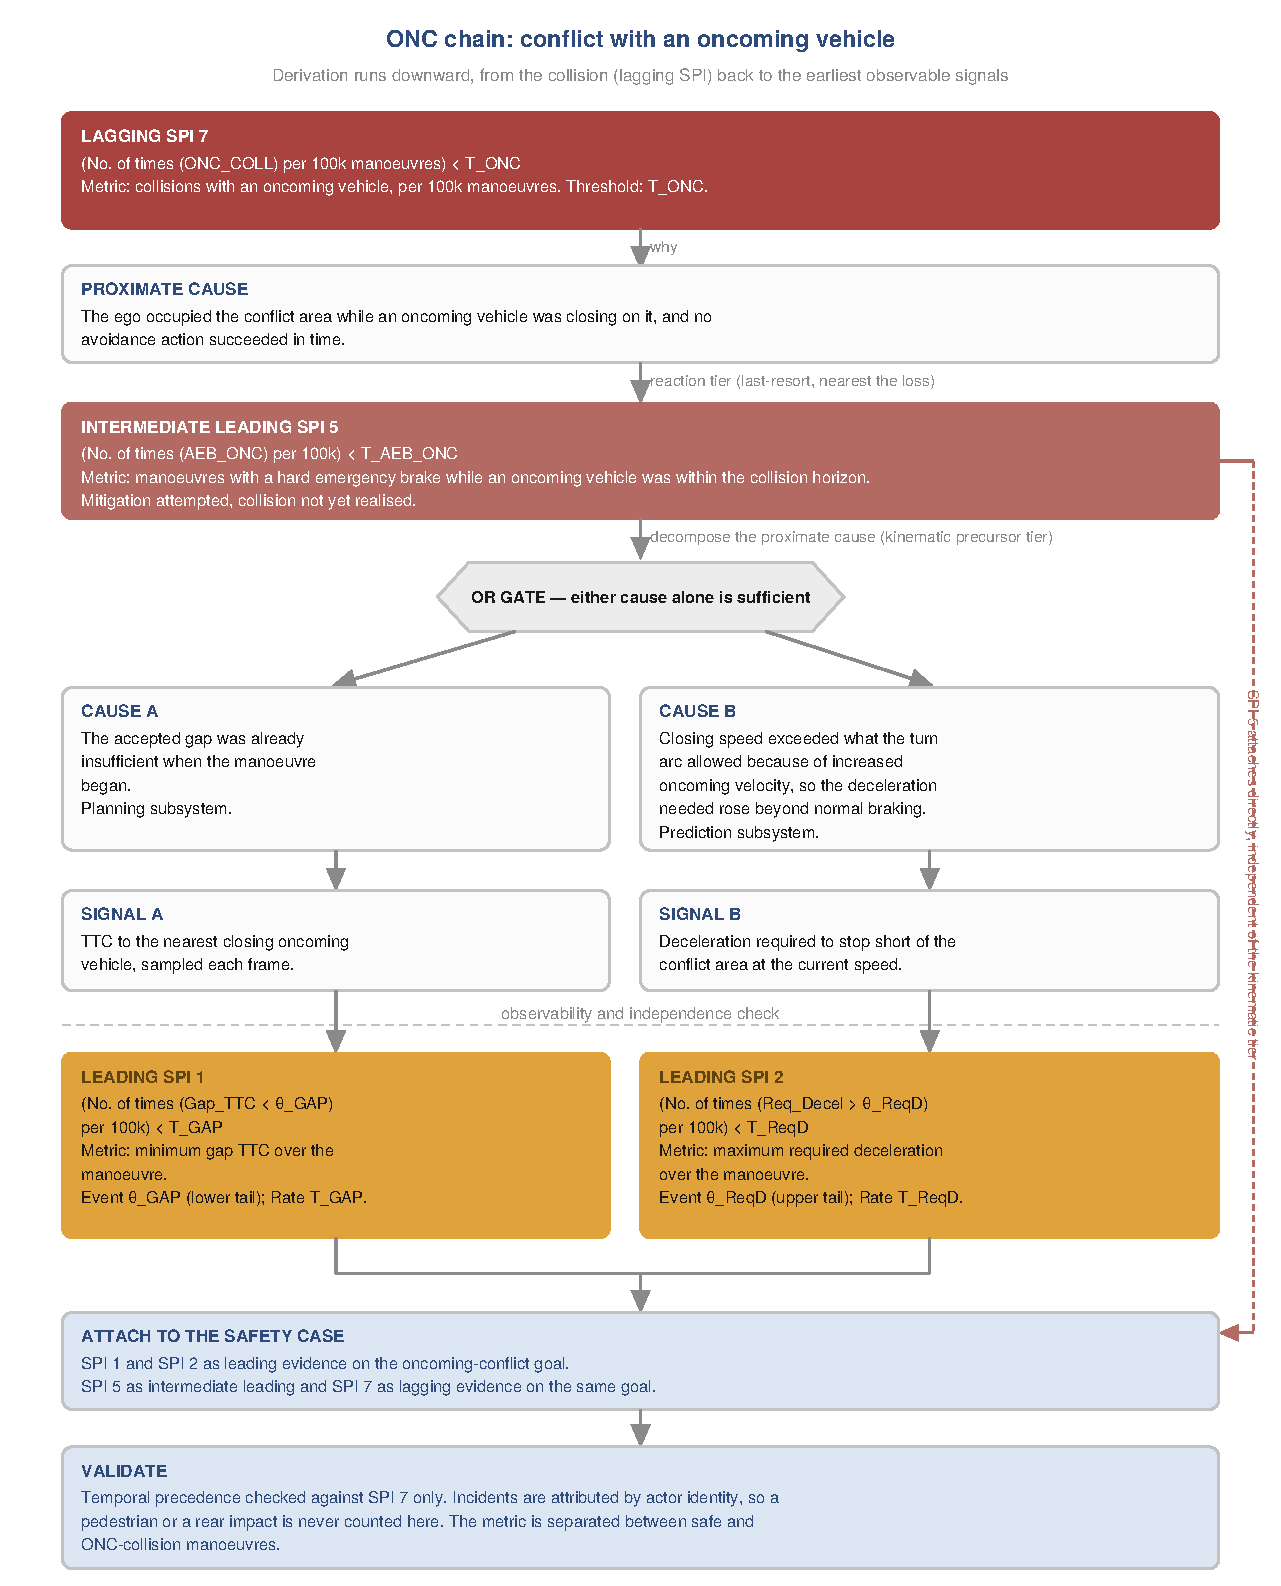
\includegraphics[width=15cm]{spi_causal_chain_example}
    \caption{Worked causal-chain derivation for the left-turn use case. The lagging
    indicator, a collision with an oncoming vehicle, is decomposed through its proximate
    cause and an OR gate into two subsystem-level intermediate causes, each yielding a
    leading indicator with its own earliest observable signal and lead time. The
    emergency-braking activation is the intermediate leading indicator of the reaction
    tier and attaches to the safety case independently of the kinematic branches.}
    \label{fig:causal_chain_example}
\end{figure}
% ---------------------------------------------------------------------------
% PASTE INTO: Chapter 4, Section 4.8 (Worked Examples)
% WHERE:      directly after the existing Figure 4.2 (the ONC chain figure)
% UPLOAD:     spi_causal_chain_ped.pdf and spi_causal_chain_rear.pdf into your Graphics folder

% First add this sentence to the end of the paragraph above Figure 4.2:
%
%   The same derivation is carried out for the other two conflict chains of the
%   manoeuvre. Figure~\ref{fig:chain_ped} gives the pedestrian chain and
%   Figure~\ref{fig:chain_rear} the following chain. The three differ in where the
%   derivation terminates: the oncoming and pedestrian chains each retain a
%   reaction-tier indicator, whereas the following chain has none, and the
%   pedestrian and following chains each lose one branch at the observability and
%   independence check of Step~5.

\begin{figure}[htbp]
  \centering
  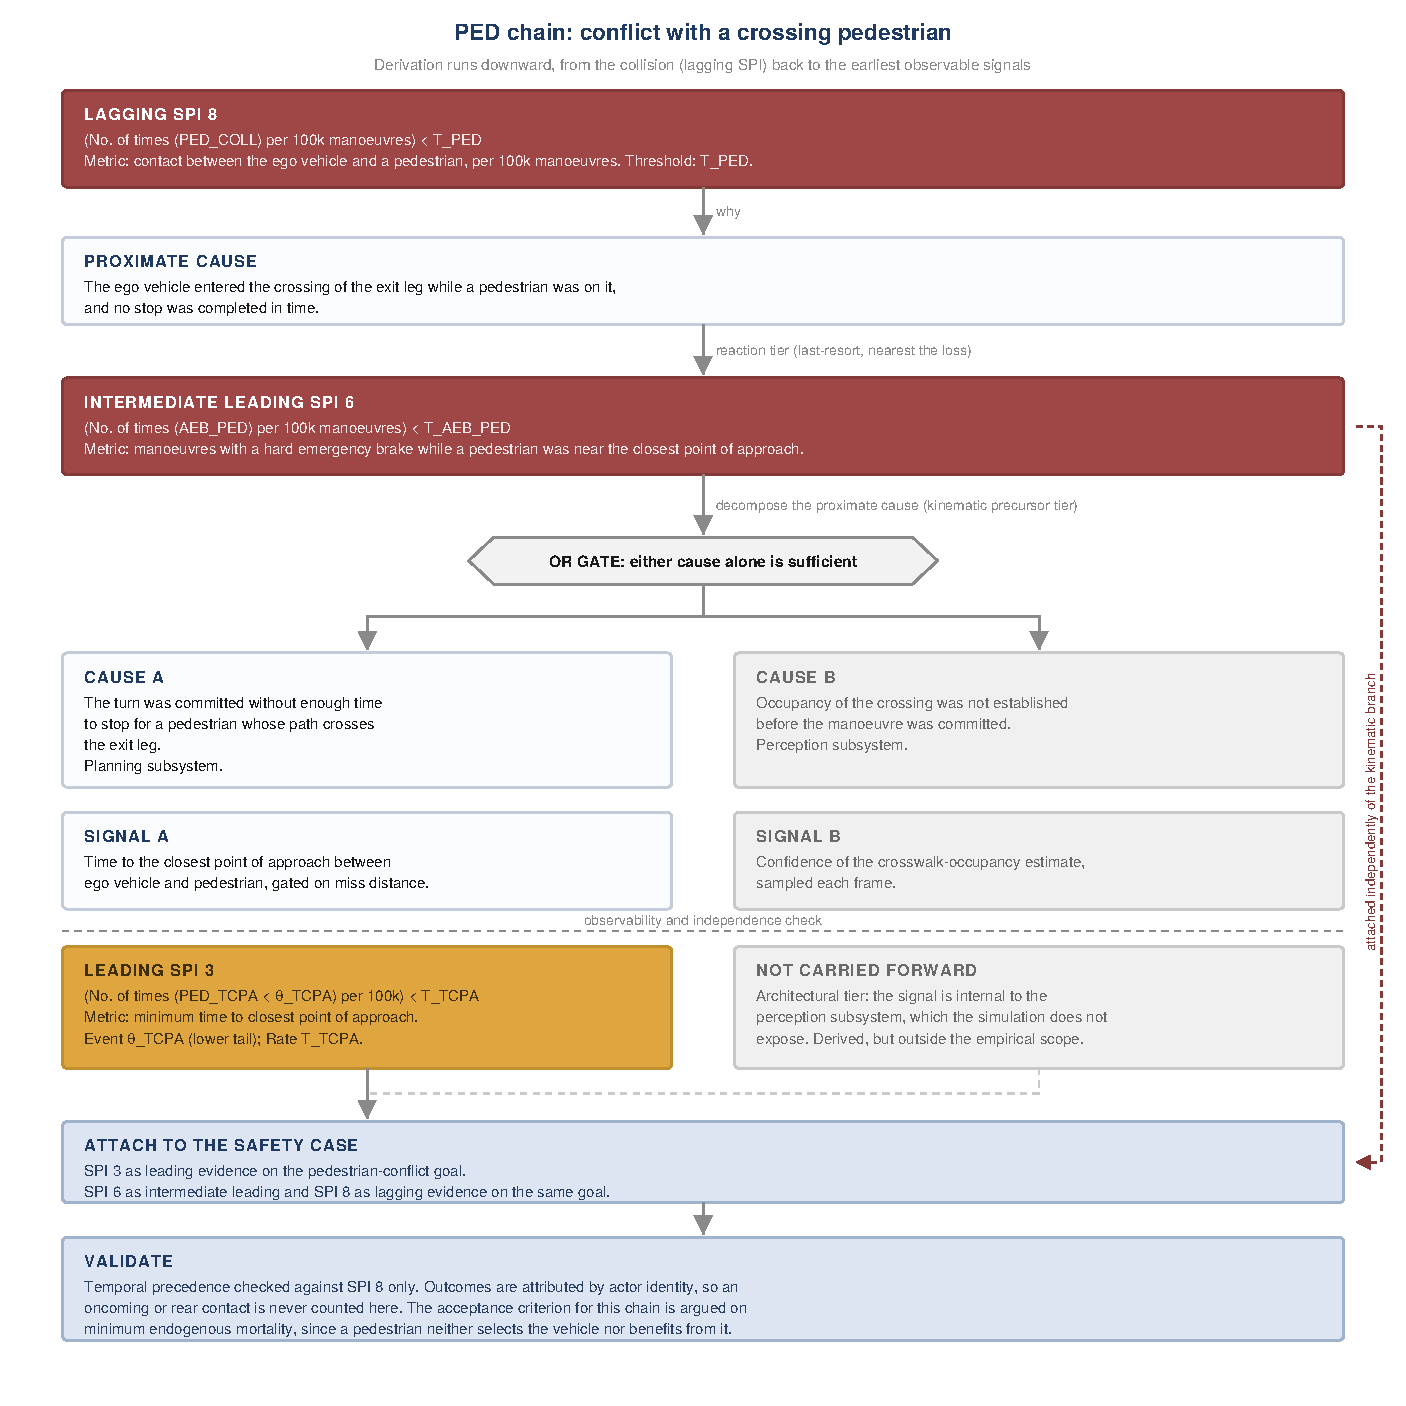
\includegraphics[width=15cm]{spi_causal_chain_ped}
  \caption{Worked causal-chain derivation for the pedestrian-crossing
    conflict. The lagging indicator, a collision with a crossing pedestrian,
    is decomposed through its proximate cause and an OR gate into two
    subsystem-level intermediate causes. Only the planning branch yields an
    indicator that survives Step~5; the perception branch is derived but is
    of the architectural tier and therefore outside the empirical scope of
    this work.}
  \label{fig:chain_ped}
\end{figure}

\begin{figure}[htbp]
  \centering
  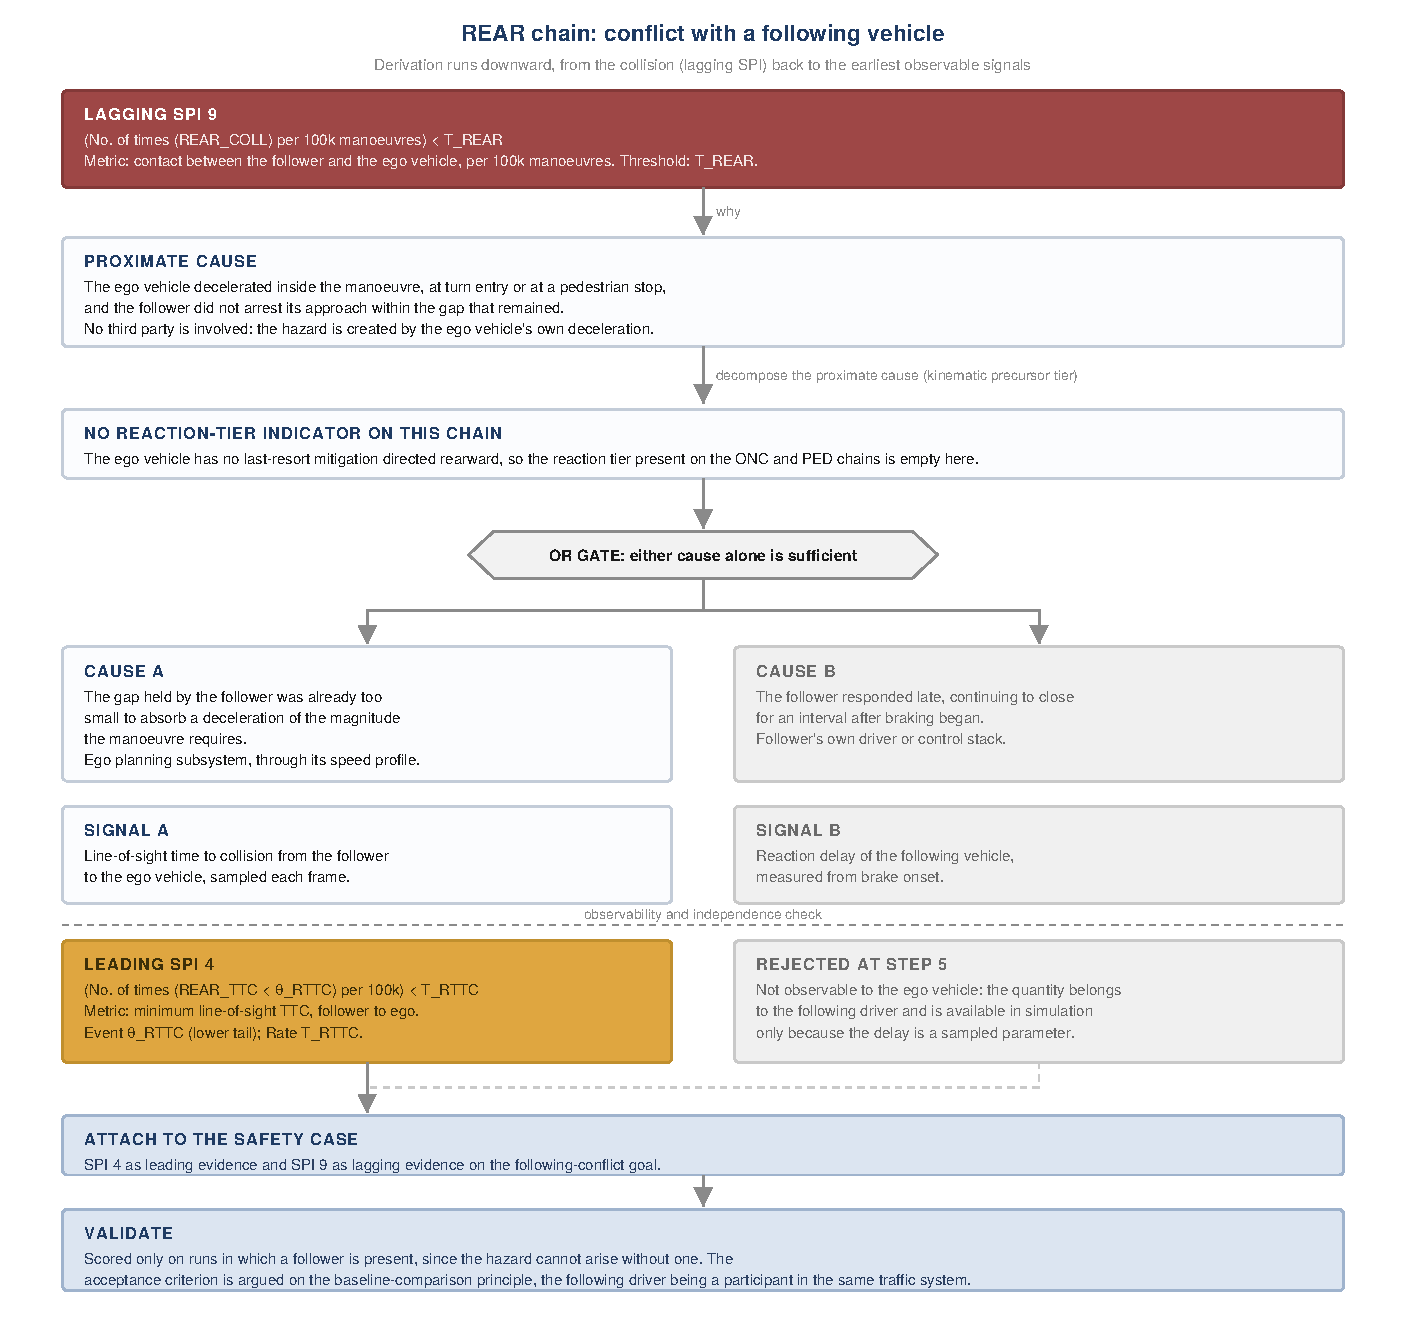
\includegraphics[width=15cm]{spi_causal_chain_rear}
  \caption{Worked causal-chain derivation for the following-vehicle conflict.
    The chain carries no reaction-tier indicator, because the ego vehicle has
    no last-resort mitigation directed rearward, and the branch attributing
    the conflict to the follower's reaction delay is rejected at Step~5 as
    not observable to the ego vehicle.}
  \label{fig:chain_rear}
\end{figure}
\section{Instantiation of the Method}
\label{sec:method_carla}

The seven steps above are defined without reference to a particular use case or
simulator, which is what allows the same procedure to be applied to the three conflict
chains of a single manoeuvre. Their instantiation is the subject of
Chapter~\ref{ch:experiment}, which fixes the simulation environment and the ego
configuration, describes each of the three conflict chains and the mechanism by which
conflicts in it are generated, states the indicator register that Steps~3 to~7 produce
for those chains, and defines the criteria against which the resulting indicators are
judged. Chapter~\ref{ch:results} then reports the evaluation against those definitions.

Two properties of the instantiation are noted here because they follow from the method
rather than from the experiment. First, because the configuration used exposes no
perception internals, every indicator that survives the observability and independence
check of Section~\ref{sec:method_signal} is of the behavioural tier; the
architectural-tier indicators that depend on detection confidence or time of first
detection are outside the empirical scope of this work, since ground truth carries no
notion of confidence and a calibrated perception model would be required before any
threshold on such a signal is meaningful. Second, indicators are computed in
post-processing rather than during a run, which permits $\theta$ and $T$ to be
recalibrated without regenerating the scenarios, and which equally means that the
runtime cost of evaluating an indicator on a vehicle is not measured here. The
operational loop of Chapter~\ref{ch:sota} is accordingly evidenced in its derivation and
monitoring stages only.
\input{Chapters/05_Experimental_Setup}
% =============================================================================
% Chapter 6: Results
% Findings only. All interpretation is in Chapter 7.
% Every figure block is copied verbatim from figure_captions.tex and every table
% from tables.tex or dashboard_tables.tex, so the numbers cannot drift.
% Results are reported as actual run counts with their eligible population;
% rates per 100,000 appear only inside an SPI definition, never as a result.
% =============================================================================

\chapter{Results}
\label{ch:results}

This chapter reports what the register of Chapter~\ref{ch:methodology} does on
the 94,816 analysed runs of Chapter~\ref{ch:experiment}. It states the findings
and does not interpret them; the interpretation follows in
Chapter~\ref{ch:discussion}. Every result is given as a number of runs together
with the eligible population of the chain concerned.

Section~\ref{sec:results_collisions} gives the collisions each chain produced.
Section~\ref{sec:results_violations} sets the violations of the leading SPIs
against those collisions, and Section~\ref{sec:results_leadtime} reports which
collisions were preceded by a violation and by how long.
Section~\ref{sec:results_statistics} gives the detection statistics.
Sections~\ref{sec:results_gate} and~\ref{sec:results_poolability} report two
properties of the evaluation itself, namely the effect of the oncoming conflict
gate and the transferability of the metric thresholds between campaigns.
Section~\ref{sec:results_dashboard} gives the state of the register as the
monitoring dashboard presents it.

% =============================================================================
\section{Collisions per Conflict Chain}
\label{sec:results_collisions}

The collisions are the reference events of the whole evaluation, so they are
stated first. Table~\ref{tab:collisions_per_chain} gives them per chain and per
campaign under the collision definition of
Section~\ref{sec:exp_collision}.

% ---------------------------------------------------------------------------
\begin{table}[htbp]
    \centering
    \caption{Collisions per conflict chain. The table counts the collision runs
    of each chain per campaign under the collision definition of
    Section~\ref{sec:exp_collision}.}
    \label{tab:collisions_per_chain}
    \small
    \begin{tabular}{@{}lrrrr@{}}
        \toprule
        {\bfseries Chain} & {\bfseries Campaign 1} & {\bfseries Campaign 2} &
        {\bfseries Campaign 3} & {\bfseries Total} \\
        \midrule
        Oncoming vehicle (ONC)  & 540 & 0 & 0 & 540 \\
        Pedestrian (PED)        & 814 & 1 & 0 & 815 \\
        Following vehicle (REAR)& 101 & 0 & 0 & 101 \\
        \bottomrule
    \end{tabular}
\end{table}

All 540 oncoming-vehicle collisions and all 101 following-vehicle collisions
occur in Campaign~1. Of the 815 pedestrian collisions, 814 occur in Campaign~1
and one in Campaign~2. The 75,509 runs of Campaigns~2 and~3 together therefore
contain a single collision across all three chains.

% =============================================================================
\section{Violations and Collisions}
\label{sec:results_violations}

The question this section answers is how often each leading SPI was violated,
set against how often its chain produced a collision, and whether that relation
survives the change from the provoked configuration to realistic driving.
Figure~\ref{fig:6_1_violations_collisions} and
Table~\ref{tab:violations_collisions} give the counts.

% ---------------------------------------------------------------------------
% Copied verbatim from figure_captions.tex
\begin{figure}[htbp]
\centering
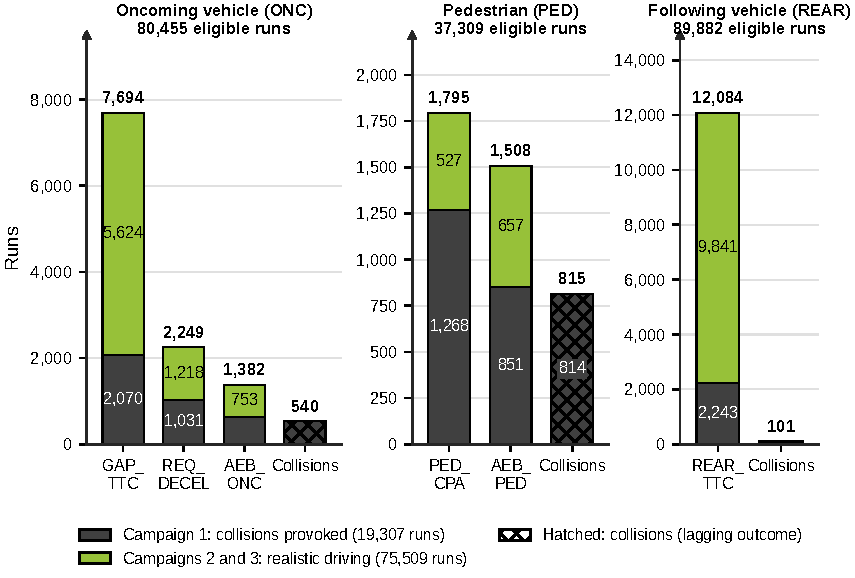
\includegraphics[width=16cm]{fig_6_1_violations_collisions.pdf}
\caption{Leading SPI violations and collisions per conflict chain. Bars give the number of eligible runs in which each leading SPI was violated and the number of collision runs of the chain (hatched), split into Campaign 1 and Campaigns 2 and 3; the metric thresholds are calibrated on Campaign 1 and applied unchanged to all 94,816 runs.}
\label{fig:6_1_violations_collisions}
\end{figure}

% ---------------------------------------------------------------------------
% Copied verbatim from tables.tex
\begin{table}[htbp]
\centering
\caption{Violations and collisions. The table gives the number of runs per configuration in which each leading SPI was violated, and the collision runs of its chain.}
\label{tab:violations_collisions}
\small
\begin{tabular}{@{}llrrrrr@{}}
\toprule
{\bfseries Indicator} & {\bfseries Chain} & {\bfseries \begin{tabular}[b]{@{}c@{}}Eligible\\runs\end{tabular}} & {\bfseries \begin{tabular}[b]{@{}c@{}}Violations\\Campaign 1\end{tabular}} & {\bfseries \begin{tabular}[b]{@{}c@{}}Violations\\Campaigns 2, 3\end{tabular}} & {\bfseries \begin{tabular}[b]{@{}c@{}}Violations\\total\end{tabular}} & {\bfseries \begin{tabular}[b]{@{}c@{}}Collisions\\C1 / C2, 3\end{tabular}} \\
\midrule
GAP\_TTC & ONC & 80,455 & 2,070 & 5,624 & 7,694 & 540 / 0 \\
REQ\_DECEL & ONC & 80,455 & 1,031 & 1,218 & 2,249 & 540 / 0 \\
AEB\_ONC & ONC & 80,455 & 629 & 753 & 1,382 & 540 / 0 \\
PED\_CPA & PED & 37,309 & 1,268 & 527 & 1,795 & 814 / 1 \\
AEB\_PED & PED & 37,309 & 851 & 657 & 1,508 & 814 / 1 \\
REAR\_TTC & REAR & 89,882 & 2,243 & 9,841 & 12,084 & 101 / 0 \\
\bottomrule
\end{tabular}
\end{table}

The eligible populations differ between the two configurations. For the oncoming
chain, 15,362 of the 80,455 eligible runs belong to Campaign~1 and 65,093 to
Campaigns~2 and~3; for the pedestrian chain, 8,424 and 28,885; for the
following-vehicle chain, 14,373 and 75,509.

In Campaign~1 the violation counts and the collision counts are of the same
order. The oncoming chain records 2,070 GAP\_TTC violations against 540
collisions, which is 3.8 violations per collision, 1,031 REQ\_DECEL violations at
1.9 per collision and 629 AEB\_ONC events at 1.2 per collision. The pedestrian
chain records 1,268 PED\_CPA violations against 814 collisions, or 1.6 per
collision, and 851 AEB\_PED events at 1.0 per collision. The following-vehicle
chain records 2,243 REAR\_TTC violations against 101 collisions, or 22.2 per
collision.

In Campaigns~2 and~3 the relation changes. The 75,509 runs contain one collision,
while every leading SPI continues to be violated: 5,624 times for GAP\_TTC, 1,218
for REQ\_DECEL, 753 for AEB\_ONC, 527 for PED\_CPA, 657 for AEB\_PED and 9,841
for REAR\_TTC. For the pedestrian chain this gives 527 PED\_CPA violations and
657 AEB\_PED events per collision. For the chains without any collision no ratio
is defined; using the 95\,\% Wilson upper bound of a zero collision count gives
at least 1,464 violations per collision for GAP\_TTC, at least 317 for
REQ\_DECEL, at least 196 for AEB\_ONC and at least 2,562 for REAR\_TTC.

% =============================================================================
\section{Detection and Lead Time}
\label{sec:results_leadtime}

A violation is only useful if it precedes the collision it anticipates, and the
time by which it precedes it bounds any response. This section reports both.
Figure~\ref{fig:6_2_detection} gives the share of collision runs with an earlier
violation, Figure~\ref{fig:6_3_lead_time} the distribution of the lead time, and
Table~\ref{tab:lead_time} both as counts. Lead time is measured from the first
violation in the run to the collision.

% ---------------------------------------------------------------------------
% Copied verbatim from figure_captions.tex
\begin{figure}[htbp]
\centering
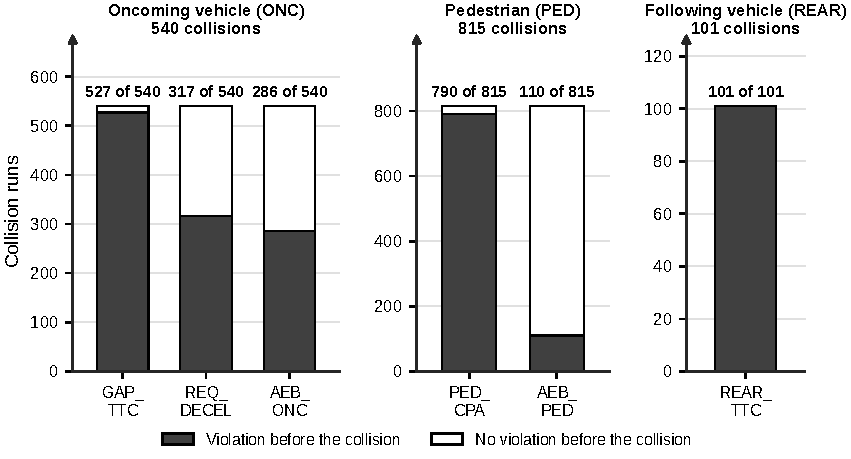
\includegraphics[width=16cm]{fig_6_2_detection.pdf}
\caption{Collision runs with a violation before the collision. For each leading SPI, the bar divides the collision runs of its chain into runs in which the SPI was violated before the collision and runs without such a violation, over all 94,816 analysed runs.}
\label{fig:6_2_detection}
\end{figure}

% ---------------------------------------------------------------------------
% Copied verbatim from figure_captions.tex
\begin{figure}[htbp]
\centering
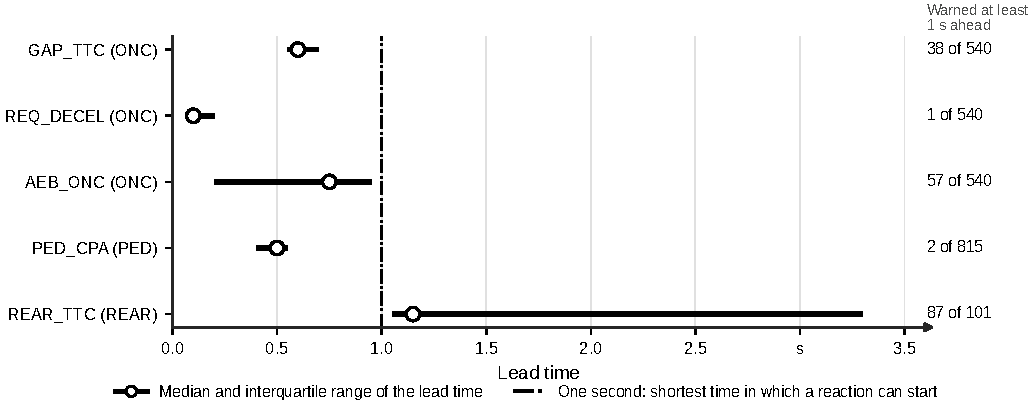
\includegraphics[width=16cm]{fig_6_3_lead_time.pdf}
\caption{Lead time of the leading SPIs. Markers give the median and bars the interquartile range of the time from the first violation to the collision in collision runs with an earlier violation; the numbers at the right count collisions warned at least 1\,s ahead. AEB\_PED is omitted because its lead time does not measure a warning.}
\label{fig:6_3_lead_time}
\end{figure}

% ---------------------------------------------------------------------------
% Copied verbatim from tables.tex
\begin{table}[htbp]
\centering
\caption{Detection and lead time. The table counts collision runs with an earlier violation and gives the time from the first violation to the collision.}
\label{tab:lead_time}
\small
\begin{tabular}{@{}llrrrr@{}}
\toprule
{\bfseries Indicator} & {\bfseries Chain} & {\bfseries \begin{tabular}[b]{@{}c@{}}Violation before\\collision\end{tabular}} & {\bfseries \begin{tabular}[b]{@{}c@{}}Median\\lead\end{tabular}} & {\bfseries Q1 to Q3} & {\bfseries \begin{tabular}[b]{@{}c@{}}Warned at least\\1\,s ahead\end{tabular}} \\
\midrule
GAP\_TTC & ONC & 527 of 540 & 0.60\,s & 0.55 to 0.70\,s & 38 of 540 \\
REQ\_DECEL & ONC & 317 of 540 & 0.10\,s & 0.10 to 0.20\,s & 1 of 540 \\
AEB\_ONC & ONC & 286 of 540 & 0.75\,s & 0.20 to 0.95\,s & 57 of 540 \\
PED\_CPA & PED & 790 of 815 & 0.50\,s & 0.40 to 0.55\,s & 2 of 815 \\
AEB\_PED & PED & 110 of 815 & 5.15\,s & 4.95 to 6.24\,s & not a warning time \\
REAR\_TTC & REAR & 101 of 101 & 1.15\,s & 1.05 to 3.30\,s & 87 of 101 \\
\bottomrule
\end{tabular}
\par\smallskip\footnotesize\raggedright Lead time is measured from the first violation in the run.
\end{table}

The two kinematic indicators that watch the first branch of their chain precede
nearly every collision of that chain: GAP\_TTC 527 of 540 oncoming-vehicle
collisions, PED\_CPA 790 of 815 pedestrian collisions and REAR\_TTC all 101
following-vehicle collisions. REQ\_DECEL precedes 317 of 540 and AEB\_ONC 286 of
540 oncoming-vehicle collisions. AEB\_PED precedes 110 of 815 pedestrian
collisions.

The lead times separate the following conflict from the two crossing conflicts.
REAR\_TTC has a median lead of 1.15\,s and warns at least one second ahead in 87
of the 101 following-vehicle collisions. The three oncoming-vehicle indicators
have median leads of 0.60\,s, 0.10\,s and 0.75\,s and warn at least one second
ahead in 38, one and 57 of the 540 collisions respectively. PED\_CPA has a median
lead of 0.50\,s and warns at least one second ahead in two of the 815 pedestrian
collisions.

The AEB\_PED row is not comparable with the others. Only 110 of the 815
pedestrian collisions follow an emergency braking event at all, and in those 110
runs the event lies between 4.95\,s and 6.24\,s before the collision, with a
median of 5.15\,s. Because lead time is measured from the first violation
anywhere in the run, this interval is not established to be a warning time for
the collision that follows it, and it is not reported as one. The point is taken
up in Section~\ref{sec:disc_aebped}.

% =============================================================================
\section{Detection Statistics}
\label{sec:results_statistics}

The counts of the previous section describe each indicator from one side at a
time. This section combines them into the classification of
Section~\ref{sec:exp_criteria} and reports precision, recall, false-alarm rate
and relative risk with their intervals. Table~\ref{tab:confusion_counts} gives
the classification of every eligible run and
Table~\ref{tab:detection_statistics} the measures derived from it.

% ---------------------------------------------------------------------------
% Copied verbatim from tables.tex
\begin{table}[htbp]
\centering
\caption{Confusion counts. The table classifies every eligible run by whether the SPI was violated before any collision and whether a collision of the chain occurred.}
\label{tab:confusion_counts}
\small
\begin{tabular}{@{}llrrrr@{}}
\toprule
{\bfseries Indicator} & {\bfseries Chain} & {\bfseries TP} & {\bfseries FP} & {\bfseries FN} & {\bfseries TN} \\
\midrule
GAP\_TTC & ONC & 527 & 7,167 & 13 & 72,748 \\
REQ\_DECEL & ONC & 317 & 1,932 & 223 & 77,983 \\
AEB\_ONC & ONC & 286 & 1,096 & 254 & 78,819 \\
PED\_CPA & PED & 790 & 1,005 & 25 & 35,489 \\
AEB\_PED & PED & 110 & 1,398 & 705 & 35,096 \\
REAR\_TTC & REAR & 101 & 11,983 & 0 & 77,798 \\
\bottomrule
\end{tabular}
\par\smallskip\footnotesize\raggedright TP: violation before a collision of the chain; FP: violation, no collision; FN: collision without an earlier violation; TN: neither.
\end{table}

% ---------------------------------------------------------------------------
% Copied verbatim from tables.tex
\begin{table}[htbp]
\centering
\caption{Detection statistics. Precision, recall, false-alarm rate and relative risk of each leading SPI over all eligible runs, with 95\,\% intervals.}
\label{tab:detection_statistics}
\footnotesize
\setlength{\tabcolsep}{4pt}
\begin{tabular}{@{}lrrrr@{}}
\toprule
{\bfseries Indicator} & {\bfseries \begin{tabular}[b]{@{}c@{}}Precision\\in \%\end{tabular}} & {\bfseries \begin{tabular}[b]{@{}c@{}}Recall\\in \%\end{tabular}} & {\bfseries \begin{tabular}[b]{@{}c@{}}False-alarm\\rate in \%\end{tabular}} & {\bfseries Relative risk} \\
\midrule
GAP\_TTC & 6.8 [6.3, 7.4] & 97.6 [95.9, 98.6] & 8.97 & 383.4 [221.2, 664.3] \\
REQ\_DECEL & 14.1 [12.7, 15.6] & 58.7 [54.5, 62.8] & 2.42 & 49.4 [41.9, 58.4] \\
AEB\_ONC & 20.7 [18.6, 22.9] & 53.0 [48.7, 57.1] & 1.37 & 64.4 [54.9, 75.6] \\
PED\_CPA & 44.0 [41.7, 46.3] & 96.9 [95.5, 97.9] & 2.75 & 625.2 [421.1, 928.3] \\
AEB\_PED & 7.3 [6.1, 8.7] & 13.5 [11.3, 16.0] & 3.83 & 3.7 [3.1, 4.5] \\
REAR\_TTC & 0.8 [0.7, 1.0] & 100.0 [96.3, 100.0] & 13.35 & $\geq$\,1,306.8 [81.2, 21,035.8] \\
\bottomrule
\end{tabular}
\par\smallskip\footnotesize\raggedright Precision and recall with Wilson score intervals; relative risk with the Katz log interval. REAR\_TTC: every collision was preceded by a violation, so the relative risk is a Haldane-corrected lower bound.
\end{table}

Every leading SPI has a relative risk whose 95\,\% interval excludes unity. The
point estimates are 383.4 for GAP\_TTC, 49.4 for REQ\_DECEL, 64.4 for AEB\_ONC,
625.2 for PED\_CPA and 3.7 for AEB\_PED; REAR\_TTC records no collision without
an earlier violation, so its value of 1,306.8 is a lower bound and its interval,
from 81.2 to 21,035.8, is correspondingly wide.

The pooled precision values rest on all three campaigns together, and
Campaigns~2 and~3 contribute violations while contributing one collision. The
pooled precision is therefore lower than the precision within Campaign~1 for
every indicator, and the two values are reported together.
Table~\ref{tab:statistics_per_campaign}, placed in Appendix~\ref{app:statistics},
gives the full per-campaign breakdown. Within Campaign~1 the precision is
25.5\,\% for GAP\_TTC against 6.8\,\% pooled, 30.7\,\% against 14.1\,\% for
REQ\_DECEL, 45.5\,\% against 20.7\,\% for AEB\_ONC, 62.2\,\% against 44.0\,\%
for PED\_CPA, 12.8\,\% against 7.3\,\% for AEB\_PED and 4.5\,\% against 0.8\,\%
for REAR\_TTC. The relative risks within Campaign~1 are 260.3 for GAP\_TTC, 19.8
for REQ\_DECEL, 26.4 for AEB\_ONC, 178.1 for PED\_CPA, 1.4 for AEB\_PED and at
least 1,097.4 for REAR\_TTC.

% =============================================================================
\section{Effect of the Oncoming Conflict Gate}
\label{sec:results_gate}

Step~5 of the derivation requires that an indicator be computed only where its
conflict can arise. For the oncoming chain this is implemented by the conflict
gate defined in Chapter~\ref{ch:methodology}, and its effect is isolated by scoring the
three oncoming-vehicle indicators twice on the same runs, once with and once
without the gate. Table~\ref{tab:conflict_gate} gives the comparison.

% ---------------------------------------------------------------------------
% Copied verbatim from tables.tex
\begin{table}[htbp]
\centering
\caption{Oncoming conflict gate. The table compares the oncoming chain without and with the conflict gate.}
\label{tab:conflict_gate}
\small
\begin{tabular}{@{}lrrr@{}}
\toprule
{\bfseries Indicator} & {\bfseries Eligible runs} & {\bfseries Violations} & {\bfseries ONC collisions} \\
\midrule
GAP\_TTC & 94,816 / 80,455 & 10,360 / 7,694 & 540 / 540 \\
REQ\_DECEL & 94,816 / 80,455 & 3,146 / 2,249 & 540 / 540 \\
AEB\_ONC & 94,816 / 80,455 & 1,490 / 1,382 & 540 / 540 \\
\bottomrule
\end{tabular}
\par\smallskip\footnotesize\raggedright Values given as without gate / with gate.
\end{table}

The gate removes 14,361 runs from the eligible population of the oncoming chain
and all 540 oncoming-vehicle collisions remain eligible. The violation counts
fall from 10,360 to 7,694 for GAP\_TTC, from 3,146 to 2,249 for REQ\_DECEL and
from 1,490 to 1,382 for AEB\_ONC.

% =============================================================================
\section{Poolability of the Metric Thresholds}
\label{sec:results_poolability}

The metric thresholds are calibrated on Campaign~1 and applied to all three
campaigns, which is defensible only if the underlying distributions are close
enough for one value to stand for all of them. To test this, each threshold was
recalibrated separately on each campaign and the pairwise relative shift
examined. Table~\ref{tab:poolability} gives the result; pooling is refused above
a relative shift of 15\,\%.

% ---------------------------------------------------------------------------
% Copied verbatim from tables.tex
\begin{table}[htbp]
\centering
\caption{Threshold poolability. Metric thresholds calibrated separately per campaign and their relative shift.}
\label{tab:poolability}
\small
\begin{tabular}{@{}lrrrrrr@{}}
\toprule
{\bfseries Indicator} & {\bfseries $\theta$ C1} & {\bfseries $\theta$ C2} & {\bfseries $\theta$ C3} & {\bfseries Shift 1 vs 2} & {\bfseries Shift 1 vs 3} & {\bfseries Shift 2 vs 3} \\
\midrule
GAP\_TTC & 0.913 & 0.927 & 0.926 & 1.55\,\% & 1.50\,\% & 0.05\,\% \\
REQ\_DECEL & 7.549 & 5.924 & 5.924 & 21.52\,\%, no & 21.52\,\%, no & 0.00\,\% \\
PED\_CPA & 1.174 & 1.619 & 1.617 & 37.90\,\%, no & 37.74\,\%, no & 0.12\,\% \\
REAR\_TTC & 2.679 & 2.517 & 2.500 & 6.08\,\% & 6.71\,\% & 0.67\,\% \\
\bottomrule
\end{tabular}
\par\smallskip\footnotesize\raggedright Pooling is refused above 15\,\% relative shift (marked no).
\end{table}

Campaigns~2 and~3 agree on every metric threshold to within 0.67\,\%, so
Campaign~3 is a statistical replicate of Campaign~2. Between Campaign~1 and the
two realistic-driving campaigns, the thresholds of GAP\_TTC and REAR\_TTC remain
within the criterion, at shifts of 1.55\,\% and 1.50\,\% and of 6.08\,\% and
6.71\,\%. The thresholds of REQ\_DECEL and PED\_CPA do not: REQ\_DECEL shifts by
21.52\,\% against both campaigns and PED\_CPA by 37.90\,\% and 37.74\,\%.

% =============================================================================
\section{The Register under Monitoring}
\label{sec:results_dashboard}

The preceding sections evaluate the register after the fact. A monitoring process
reads it while the runs accumulate, and the form in which it does so is part of
the result. The nine SPIs were exported to a database and presented in a Grafana
dashboard; Figure~\ref{fig:6_5_dashboard} shows it. The dashboard is not deployed
on a vehicle.

% ---------------------------------------------------------------------------
\begin{figure}[htbp]
    \centering
    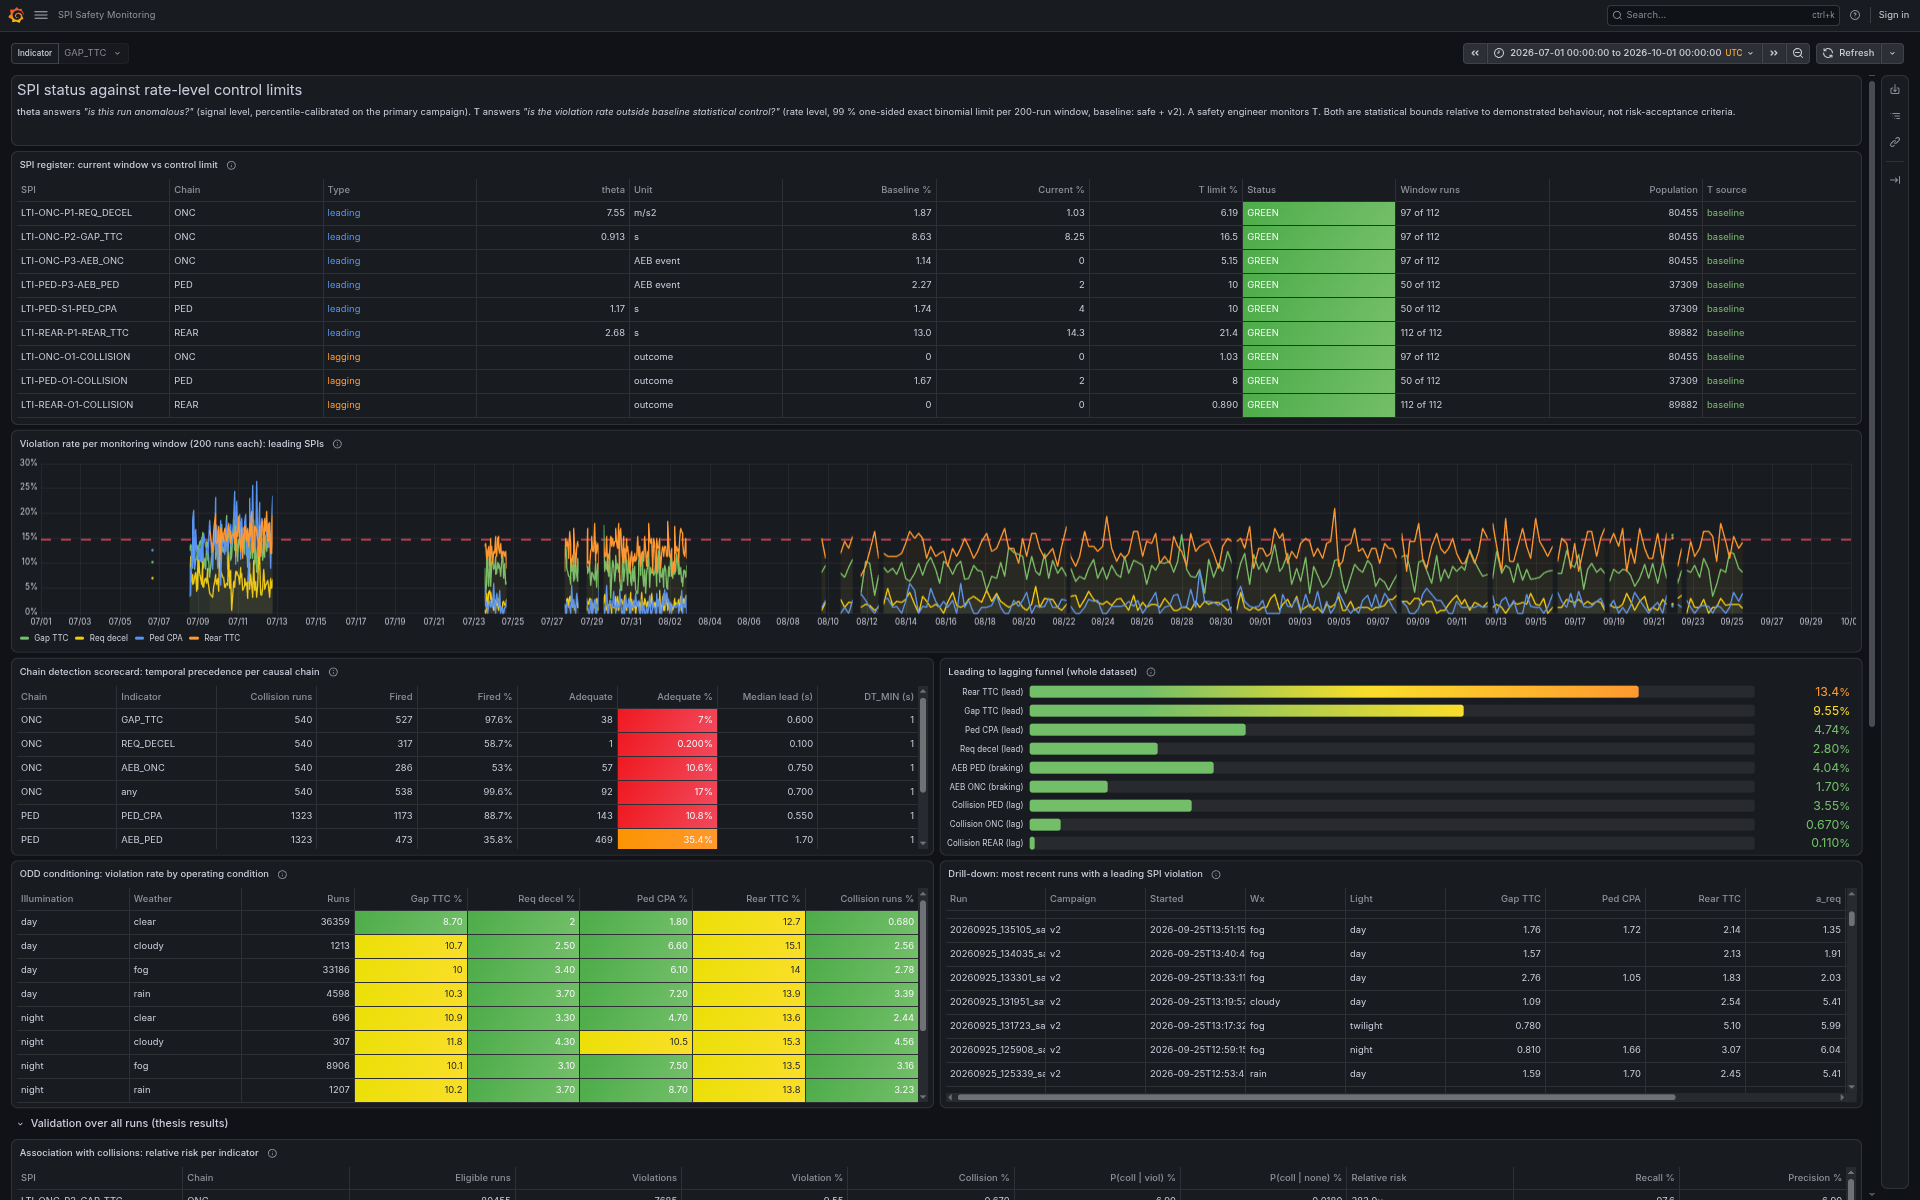
\includegraphics[width=16cm]{fig_6_5_dashboard.png}
    \caption{The SPI register under monitoring. The dashboard presents each
    indicator with its metric threshold, the baseline violations of
    Campaigns~2 and~3, a detection scorecard per chain and a funnel from
    eligible runs to collisions, over the same results as the preceding
    sections.}
    \label{fig:6_5_dashboard}
\end{figure}

The dashboard presents the register itself, a detection scorecard per chain, a
funnel from eligible runs to collisions, and tables of violations and collisions
per operating condition.
Tables~\ref{tab:dashboard_register} to~\ref{tab:dashboard_funnel} give the three
of these that bear on the register as a whole;
Table~\ref{tab:dashboard_odd}, in Appendix~\ref{app:statistics}, gives the
operating-condition breakdown.

% ---------------------------------------------------------------------------
% Trimmed from dashboard_tables.tex (v4: window columns removed)
\begin{table}[htbp]
\centering
\caption{SPI register as monitored. Identifier, type and metric threshold of each SPI, together with its baseline violations in Campaigns~2 and~3.}
\label{tab:dashboard_register}
\small
\begin{tabular}{@{}llrr@{}}
\toprule
{\bfseries SPI} & {\bfseries Type} & {\bfseries $\theta$} & {\bfseries \begin{tabular}[b]{@{}c@{}}Baseline\\(Campaigns 2, 3)\end{tabular}} \\
\midrule
LTI-ONC-P1-REQ\_DECEL & leading & 7.549\,m/s\textsuperscript{2} & 1,218 of 65,093 \\
LTI-ONC-P2-GAP\_TTC & leading & 0.913\,s & 5,624 of 65,093 \\
LTI-ONC-P3-AEB\_ONC & leading & -- & 753 of 65,093 \\
LTI-PED-P3-AEB\_PED & leading & -- & 657 of 28,885 \\
LTI-PED-S1-PED\_CPA & leading & 1.174\,s & 527 of 28,885 \\
LTI-REAR-P1-REAR\_TTC & leading & 2.679\,s & 9,841 of 75,509 \\
LTI-ONC-O1-COLLISION & lagging & -- & 0 of 65,093 \\
LTI-PED-O1-COLLISION & lagging & -- & 1 of 28,885 \\
LTI-REAR-O1-COLLISION & lagging & -- & 0 of 75,509 \\
\bottomrule
\end{tabular}
\par\smallskip\footnotesize\raggedright Baseline: eligible runs of Campaigns~2 and~3 with a violation of the SPI; lagging rows count collisions. The SPI threshold T of each indicator is derived from this baseline as defined in Equation~(\ref{eq:exp_spithreshold}).
\end{table}

The register holds nine SPIs, six leading and three lagging, each identified by
use case, chain, tier and signal. In the baseline of Campaigns~2 and~3 the six
leading SPIs record between 527 and 9,841 violating runs, whereas the three
lagging SPIs record one collision in total, which belongs to the pedestrian
chain.

% ---------------------------------------------------------------------------
% Copied verbatim from dashboard_tables.tex
\begin{table}[htbp]
\centering
\caption{Chain detection scorecard. Collision runs of each chain with a violation before the collision, for each SPI and for any SPI of the chain.}
\label{tab:dashboard_scorecard}
\small
\begin{tabular}{@{}llrrrr@{}}
\toprule
{\bfseries Chain} & {\bfseries Indicator} & {\bfseries \begin{tabular}[b]{@{}c@{}}Collision\\runs\end{tabular}} & {\bfseries \begin{tabular}[b]{@{}c@{}}Violation before\\collision\end{tabular}} & {\bfseries \begin{tabular}[b]{@{}c@{}}Lead at\\least 1\,s\end{tabular}} & {\bfseries \begin{tabular}[b]{@{}c@{}}Median\\lead\end{tabular}} \\
\midrule
ONC & GAP\_TTC & 540 & 527 & 38 & 0.60\,s \\
ONC & REQ\_DECEL & 540 & 317 & 1 & 0.10\,s \\
ONC & AEB\_ONC & 540 & 286 & 57 & 0.75\,s \\
ONC & any ONC & 540 & 538 & 92 & 0.70\,s \\
PED & PED\_CPA & 815 & 790 & 2 & 0.50\,s \\
PED & AEB\_PED & 815 & 110 & 108 & 5.15\,s \\
PED & any PED & 815 & 791 & 110 & 0.55\,s \\
REAR & REAR\_TTC & 101 & 101 & 87 & 1.15\,s \\
REAR & any REAR & 101 & 101 & 87 & 1.15\,s \\
\bottomrule
\end{tabular}
\par\smallskip\footnotesize\raggedright \emph{any}: earliest violation among the chain's indicators.
\end{table}

Taking the earliest violation among the indicators of a chain raises the
detection beyond that of any single indicator for the oncoming and pedestrian
chains: 538 of 540 oncoming-vehicle collisions and 791 of 815 pedestrian
collisions are preceded by a violation of at least one indicator of the chain,
against 527 and 790 for the best single indicator. The number warned at least one
second ahead rises from 57 to 92 for the oncoming chain and from two to 110 for
the pedestrian chain.

% ---------------------------------------------------------------------------
% Copied verbatim from dashboard_tables.tex
\begin{table}[htbp]
\centering
\caption{Leading-to-lagging funnel. Eligible runs of each chain with at least one kinematic leading violation, an emergency braking event and a collision.}
\label{tab:dashboard_funnel}
\small
\begin{tabular}{@{}lrrrr@{}}
\toprule
{\bfseries Chain} & {\bfseries Eligible runs} & {\bfseries \begin{tabular}[b]{@{}c@{}}Leading\\violation\end{tabular}} & {\bfseries \begin{tabular}[b]{@{}c@{}}Emergency\\braking\end{tabular}} & {\bfseries Collision} \\
\midrule
Oncoming vehicle & 80,455 & 9,156 & 1,382 & 540 \\
Pedestrian & 37,309 & 1,795 & 1,508 & 815 \\
Following vehicle & 89,882 & 12,084 & 0 & 101 \\
\bottomrule
\end{tabular}
\end{table}

The funnel narrows at every stage for the oncoming chain, from 80,455 eligible
runs through 9,156 with a kinematic leading violation and 1,382 with an emergency
braking event to 540 collisions. For the pedestrian chain the two leading stages
are of similar size, 1,795 and 1,508, against 815 collisions. The
following-vehicle chain has no reaction tier, so its funnel runs from 89,882
eligible runs through 12,084 leading violations to 101 collisions.
% CHANGED: 07_DiscussionConclusion + 08_Conclusion duplicated the conclusion.
% FAPS keeps Discussion and Conclusion as separate chapters. If you would
% rather merge them, delete the 08 line and rename 07 back.
% =============================================================================
% Chapter 7: Discussion
% Interprets the findings of Chapter 6. Items marked as open checks in the
% handover are presented as interpretations, not as findings.
% =============================================================================

\chapter{Discussion}
\label{ch:discussion}

Chapter~\ref{ch:results} states what the register does on 94,816 simulated left
turns. This chapter asks what those findings establish and what they do not.

Section~\ref{sec:disc_scope} fixes the scope of the claim. The three sections
that follow interpret the main findings: why leading indicators are needed at all
(Section~\ref{sec:disc_leading}), what separates an indicator that tracks the
configuration from one that tracks exposure (Section~\ref{sec:disc_exposure}),
and why the conflict geometry decides the warning time
(Section~\ref{sec:disc_geometry}). Sections~\ref{sec:disc_pedrule}
to~\ref{sec:disc_threshold} discuss four individual decisions and anomalies: the
pedestrian collision rule, the behaviour of AEB\_PED and the reaction tier, the
formulation of REQ\_DECEL, and the choice of metric threshold.
Section~\ref{sec:disc_limitations} collects the limitations.

% =============================================================================
\section{What the Results Validate}
\label{sec:disc_scope}

The scope of the claim has to be stated before the findings are interpreted,
because the evaluation is easily read as saying more than it does.

The results validate the derivation method and the evaluation, not the safety of
a driving function. The ego vehicle is driven by the CARLA Traffic Manager with a
pedestrian-stop rule and without gap acceptance, so the conflicts that arise in
the oncoming chain follow from a capability the vehicle does not have rather than
from a functional insufficiency of a system that has it. The indicators are
computed from logged ground truth rather than from a perceived world model. What
the evaluation therefore shows is that the signals the method derives behave as
precursors of the collisions they were derived from, under a controlled and
reproducible exposure. It shows nothing about how safe the simulated vehicle is,
and a collision count obtained under a generator built to provoke collisions
carries no information about collision frequency in operation.

% =============================================================================
\section{Why Leading Indicators Are Needed}
\label{sec:disc_leading}

The argument for leading indicators is usually made in principle, by observing
that losses are too rare to count. The two configurations evaluated here allow it
to be made with measurements instead, because they place the same register in
both regimes.

In Campaign~1 the leading SPIs and the collisions are of comparable size. The
oncoming chain records 3.8 GAP\_TTC violations, 1.9 REQ\_DECEL violations and 1.2
AEB\_ONC events per collision, and the pedestrian chain 1.6 PED\_CPA violations
and 1.0 AEB\_PED events per collision. In that regime the lagging indicator is
itself countable, and a monitoring process would gain little from the leading
one.

In Campaigns~2 and~3 the position reverses. Across 75,509 runs a single collision
occurs, while the leading SPIs continue to be violated between 527 and 9,841
times. A process that monitored only the lagging indicator would have almost
nothing to observe, whereas every leading SPI still produces a measurable
quantity. This is the regime in which operational monitoring actually takes
place, and it is the regime in which the leading indicator is the only thing left
to measure.

The pattern is the precursor relation that underlies pyramid models of accident
causation [CITATION NEEDED: Heinrich's accident pyramid], and it is the rationale
for estimating rare-event frequencies from precursors \cite{bieryi1995}. The
results also show why the ratio in such models cannot be treated as a constant.
The number of violations per collision shifts by two to three orders of magnitude
between the two configurations, from 3.8 to at least 1,464 for GAP\_TTC, from 1.6
to 527 for PED\_CPA and from 22.2 to at least 2,562 for REAR\_TTC. A fixed ratio
between precursors and losses is therefore not a property that can be assumed for
a given system; it has to be measured for the configuration in question, which is
also the conclusion of the empirical critique of the fixed-ratio pyramid
\cite{yoriomoore2018}.

% =============================================================================
\section{Exposure against Configuration}
\label{sec:disc_exposure}

Every leading SPI in the register is associated with the collisions of its own
chain, yet they do not all respond to a change in the configuration. The
distinction matters because an indicator that is attached to a safety case is
expected to move when the argued property changes.

PED\_CPA responds. Its violation count falls from 1,268 in Campaign~1 to 527 in
Campaigns~2 and~3, and the pedestrian collisions fall with it, from 814 to one.
GAP\_TTC and REAR\_TTC do not. GAP\_TTC is violated 2,070 times in Campaign~1 and
5,624 times in Campaigns~2 and~3, and REAR\_TTC 2,243 and 9,841 times, while the
collisions of both chains fall from 540 and 101 to zero. Allowing for the
different eligible populations, 15,362 against 65,093 runs for the oncoming chain
and 14,373 against 75,509 for the following-vehicle chain, the counts of these
two indicators are dominated by how often the conflict is encountered rather than
by how it is handled. Both indicators identify the dangerous runs within a
configuration, as their recall of 97.6\,\% and 100\,\% shows, and both are poor
signals of a change between configurations.

The same split appears when the violation rates of the two configurations are
set against each other, which removes the difference in eligible populations.
The violation rate of PED\_CPA in Campaign~1 is 8.25 times its rate in
Campaigns~2 and~3, whereas the corresponding ratio is 1.56 for GAP\_TTC and 1.2
for REAR\_TTC. REQ\_DECEL, AEB\_ONC and AEB\_PED lie between these extremes, at
3.59, 3.54 and 4.44. An indicator whose rate barely moves while the collisions of
its chain fall from several hundred to zero cannot, on its own, signal that the
argued property has changed, however well it separates dangerous from uneventful
runs within one configuration.

This distinction carries over directly to the SPI threshold T defined in
Section~\ref{sec:method_spithreshold}. Because T bounds the violation count of a
population of runs against a baseline rate, an indicator whose rate is dominated
by exposure moves little against T when the configuration changes, whereas an
indicator whose rate tracks the configuration moves strongly. The ratios above
therefore indicate which entries of the register are suited to rate-level
monitoring and which are suited mainly to the per-run detection reported in
Section~\ref{sec:results_statistics}.

% =============================================================================
\section{Geometry Decides the Warning Time}
\label{sec:disc_geometry}

The lead times in Table~\ref{tab:lead_time} divide the register along the
conflict geometry rather than along the indicator design, which is the most
consequential finding for the timeliness question of
Section~\ref{sec:intro_objective}.

In the two crossing conflicts the partner moves across the ego vehicle's line of
sight. Time to collision and time to the closest point of approach both depend on
the closing component of the relative motion, so they change slowly while the
paths are still separated and fall quickly only once the paths almost meet. The
median lead times of 0.60\,s for GAP\_TTC and 0.50\,s for PED\_CPA follow from
that geometry, and so does the fact that only 38 of 540 oncoming-vehicle and two
of 815 pedestrian collisions are preceded by a violation at least one second
ahead. In the following conflict the partner closes along the line of sight, the
same quantity changes monotonically throughout the approach, and 87 of 101
collisions are preceded by a violation at least one second ahead. The dependence
of a criticality metric on the geometry it is applied to is the point made in the
review of such metrics \cite{westhofen2023}, and the lead times measured here are
a quantitative instance of it.

Replacing the pedestrian time to collision by the time to the closest point of
approach was a consequence of Step~4 of the derivation, which selects the
formulation the geometry admits. The change removed alarms for pedestrians whose
path misses the vehicle, which is visible in the precision of PED\_CPA, the
highest of the register at 44.0\,\%. It did not lengthen the warning time,
because it does not change what the metric depends on. Any substantially earlier
warning for a crossing pedestrian would have to come from signals of intention
such as gait, head pose or dwell at the kerb, and those are perception
quantities, outside the behavioural tier that this work evaluates.

% =============================================================================
\section{The Pedestrian Collision Rule}
\label{sec:disc_pedrule}

The rule of Section~\ref{sec:exp_collision}, under which a pedestrian contact
counts as a collision only when the ego vehicle is moving, is a decision about
the reference event rather than about an indicator, and it deserves to be
defended as such.

Without the rule the two realistic-driving campaigns would appear to produce 481
pedestrian collisions rather than one. The appearance would be an artefact: 480
of those 481 contacts occur with a standing ego vehicle, which a CARLA walker
does not avoid. The low-collision configuration would then look dangerous for a
reason that has nothing to do with the driving behaviour under observation, and
every pedestrian indicator would be scored against the wrong events. A lagging
indicator that counts the wrong events corrupts every leading indicator derived
from it, so the first step of the derivation carries at least as much weight as
the steps that follow it.

The rule is nonetheless a judgement. The audit separates the two populations
cleanly, by ego speed, by the position of the pedestrian and by a contact impulse
that differs by about a factor of ten, and the rule is stated explicitly so that
it can be challenged. The threshold of 0.3\,m/s is still a choice, and a
sensitivity analysis under the unrestricted definition would bound how far the
pedestrian results depend on it.

% =============================================================================
\section{AEB\_PED and the Order of the Reaction Tier}
\label{sec:disc_aebped}

Two results concerning the reaction tier run against the expectation under which
it was placed in the derivation, and both are discussed here rather than treated
as settled.

AEB\_PED is the weakest entry in the register once contacts with a standing ego
vehicle are excluded. It precedes 110 of the 815 pedestrian collisions, its
relative risk is 3.7, and within Campaign~1 alone it is 1.4, which is close to no
association. An emergency brake with a pedestrian in conflict therefore carries
little information about whether that run ends in a pedestrian collision. The
reading that follows from the collision rule is that the indicator previously
appeared stronger because braking brings the vehicle to a stop and a stopped
vehicle in a walker's path is walked into, so a large part of its apparent
association was with contacts that are no longer counted.

The lead time of AEB\_PED has to be read with the same reserve. In the 110 runs
in which an event precedes a collision, it does so by between 4.95\,s and
6.24\,s, with a median of 5.15\,s. Taken at face value this would be by far the
longest warning in the register. The most likely explanation is a stop-and-go
sequence: the vehicle brakes for one pedestrian, stops, drives on, and collides
with a pedestrian later in the run, with the lead time measured from the first
violation anywhere in the run. That explanation has not been verified. Confirming
it requires a per-run check of whether the ego speed falls to near zero after the
braking event and rises again before contact, and whether the pedestrian struck
is the one braked for. Until that check is carried out the interpretation stands
as the most likely reading and not as a finding, and the figure of 5.15\,s is not
reported as a warning time.

The second anomaly concerns the ordering of the tiers. The reaction tier was
placed nearest the loss, so its lead time was expected to be the shortest of the
chain. In the oncoming chain the opposite holds: the median lead of AEB\_ONC is
0.75\,s against 0.60\,s for GAP\_TTC. Two explanations are plausible and neither
is tested here. The brake command that triggers AEB\_ONC comes from the
pedestrian-stop rule of the ego configuration and is therefore not issued in
response to the oncoming vehicle at all, so it can fire early for an unrelated
reason. Alternatively the tenth-percentile metric threshold of GAP\_TTC is tight
enough to delay the kinematic violation past the braking event. Distinguishing
the two would require the same kind of per-run attribution as the AEB\_PED check.

% =============================================================================
\section{REQ\_DECEL and the Second Branch}
\label{sec:disc_reqdecel}

REQ\_DECEL precedes 317 of the 540 oncoming-vehicle collisions, markedly fewer
than the 527 of GAP\_TTC. This is the expected consequence of the decomposition
rather than a weakness of the indicator.

The two indicators were derived from the two branches of an OR gate. GAP\_TTC
watches the accepted gap, which is the branch that applies whenever the gap was
too small from the outset. REQ\_DECEL watches the deceleration that would be
required to stop short, which is the branch that applies when the closing speed
exceeds what the turn arc allows. Each branch alone is sufficient for the
collision, so neither indicator can be expected to cover the collisions of the
other.

The formulation of REQ\_DECEL carries two assumptions that make it optimistic.
The required deceleration treats the conflict partner as stationary, so a partner
that is itself closing is not accounted for, and the range entering the
denominator is clamped at a minimum value so that the expression stays finite at
short range. The clamp produces a cluster of values near 5.41\,m/s\textsuperscript{2},
which is visible in the distribution of the metric and is an artefact of the
formulation rather than a property of the conflicts. Both assumptions bias the
required deceleration downwards and therefore make violations less frequent than
a partner-aware formulation would produce.

% =============================================================================
\section{The Choice of Metric Threshold}
\label{sec:disc_threshold}

The empirical percentile was selected in Section~\ref{sec:method_thresholds} for
reasons of independence rather than of performance, and the results allow both
sides of that choice to be stated.

Its benefit is that no metric threshold is fitted on the collisions against which
the indicators are later scored. The only collision labels available are the ones
that the evaluation uses, so any criterion that optimises a detection measure on
labelled data would have produced a circular evaluation. The percentile uses the
uneventful runs of Campaign~1 only, and the resulting thresholds were applied
unchanged to all 94,816 runs, including the two campaigns that did not
contribute to the calibration.

Its cost is equally explicit and is visible in the results. A tenth-percentile
threshold is crossed by about one tenth of uneventful runs by construction, which
is the origin of the false-alarm rate of 8.97\,\% for GAP\_TTC and 13.35\,\% for
REAR\_TTC. The metric threshold marks behaviour that is unusual relative to the
calibration population; it does not mark behaviour that is unacceptable, and
nothing in the calibration establishes a level of risk. The same holds for the
SPI threshold, which is an exact binomial limit on departure from a measured
baseline and not a risk-acceptance criterion. Deriving either from ALARP, GAMAB,
MEM or a careful and competent human driver benchmark would require inputs that
this work does not have.

% =============================================================================
\section{Limitations}
\label{sec:disc_limitations}

The preceding sections qualify individual results. This section collects the
limitations that bound the evaluation as a whole;
Table~\ref{tab:limitations} states each with its consequence and the step that
would address it.

% ---------------------------------------------------------------------------
\begin{table}[htbp]
    \centering
    \caption{Limitations of the evaluation. The table states each limitation,
    the consequence it has for the results and the step that would address it.}
    \label{tab:limitations}
    \footnotesize
    \setlength{\tabcolsep}{4pt}
    \begin{tabular}{@{}>{\raggedright\arraybackslash}p{3.4cm}>{\raggedright\arraybackslash}p{5.6cm}>{\raggedright\arraybackslash}p{4.6cm}@{}}
        \toprule
        {\bfseries Limitation} & {\bfseries Consequence} & {\bfseries Next step} \\
        \midrule
        Traffic Manager ego without gap acceptance &
        Oncoming conflicts arise from a missing capability rather than from a
        functional insufficiency in the sense of ISO~21448 \cite{iso21448} &
        A gap-accepting driving function \\
        Ground-truth signals &
        The independence of the indicators from perception holds in simulation
        only &
        Perception in the loop; architectural-tier indicators \\
        Narrow exposure &
        One scenario, one map, oncoming partners that do not yield &
        Naturalistic data; responsive partners \\
        Statistical thresholds &
        $\theta$ and T bound demonstrated behaviour; ALARP, GAMAB, MEM and the
        careful and competent human driver benchmark are named but not applied &
        A risk-acceptance SPI threshold set with safety engineers \\
        Campaign comparison &
        The campaigns differ in scenario generator as well as controller, so the
        comparison is one of known groups and not a controlled experiment &
        Controlled variation of one factor \\
        Lead-time definition &
        Lead time is measured from the first violation anywhere in the run &
        Attribution of violations to the conflict partner \\
        \bottomrule
    \end{tabular}
\end{table}

The last two limitations bear on specific results. Because the campaigns differ
in two respects at once, the contrast of Section~\ref{sec:disc_exposure} shows
that PED\_CPA tracks the difference between two configurations, not that it
tracks the controller change within it. Because lead time is measured from the
first violation anywhere in the run, the AEB\_PED interval of
Section~\ref{sec:disc_aebped} cannot be attributed to the collision that follows
it without the per-run check described there.
% =============================================================================
% Chapter 8: Conclusion and Outlook
% FAPS: at most three pages. Active voice permitted for the own contribution.
% Subjunctive permitted in the outlook only.
% =============================================================================

\chapter[Conclusion and Outlook]{Conclusion and Outlook on Indicator-Based Operational Safety Assurance}
\label{ch:conclusion}

% =============================================================================
\section{Conclusion}
\label{sec:conclusion}

Operational safety assurance requires that the claims of a safety case be kept
under observation after release, and the instrument of that observation is the
safety performance indicator. UL~4600 \cite{ul4600} and PAS~1881
\cite{pas1881} require such monitoring and give examples of indicators;
ISO~21448 \cite{iso21448} requires that functional insufficiencies be monitored
in operation without saying which quantities carry that information; and the
assurance frameworks that consume indicator values take the indicators as given.
The step between an unresolved doubt in a safety case and a named signal with a
source and a threshold was the gap this thesis addressed.

This thesis makes three contributions.

The first is the Causal Chain Derivation Method. It takes a lagging outcome that
a Goal Structuring Notation claim denies and returns a leading indicator with a
signal, a source, a metric threshold and a documented path back to the claim, in
seven traceable steps: a lagging-indicator register, a proximate cause selected
by a prevention test, a decomposition through gate logic, the earliest observable
signal in the formulation the geometry admits, an observability and independence
check, the two thresholds, and attachment to the goal that the indicator actually
monitors.

The second is an evaluation of the resulting register on 94,816 simulated
unprotected left turns across three campaigns, in which the violations of six
leading indicators are set against the 540 oncoming-vehicle, 815 pedestrian and
101 following-vehicle collisions of the same runs.

The third is the monitoring of all nine indicators against their SPI thresholds
in a dashboard built on the same results, which demonstrates the form in which a
derived register is consumed.

Table~\ref{tab:rq_answers} states what the evaluation establishes for each
research question.

% ---------------------------------------------------------------------------
\begin{table}[htbp]
    \centering
    \caption{Answers to the research questions. The table states the answer
    established by the evaluation and the evidence on which it rests.}
    \label{tab:rq_answers}
    \small
    \begin{tabular}{@{}l>{\raggedright\arraybackslash}p{1.6cm}>{\raggedright\arraybackslash}p{8.4cm}@{}}
        \toprule
        {\bfseries Research question} & {\bfseries Answer} & {\bfseries Evidence} \\
        \midrule
        RQ1 Derivation &
        Yes &
        Seven traceable steps produce the register, and the checks reject
        candidates: PLAN\_DEV as an input of the controller's own error, the
        pedestrian perception branch as architectural, and the follower reaction
        delay as not observable to the ego vehicle \\
        RQ2 Timeliness &
        Partly &
        The leading SPIs remain measurable where collisions are rare, with 527 to
        9,841 violations against one collision in 75,509 runs; but only REAR\_TTC
        warns at least one second ahead in most collisions of its chain, 87 of
        101 at a median lead of 1.15\,s \\
        RQ3 Scalability &
        Yes &
        Indicators were derived and evaluated for all three conflict chains; the
        crossing chains require the time to the closest point of approach in
        place of the time to collision \\
        \bottomrule
    \end{tabular}
\end{table}

The answer to the second question is the one that qualifies the others. In the
two crossing conflicts the median lead time is 0.60\,s for GAP\_TTC and 0.50\,s
for PED\_CPA, and at least one second of warning is reached in 38 of 540 and two
of 815 collisions respectively. Measured against an in-run response, the derived
indicators of the crossing chains are not timely. Measured against an assurance
process that reads the violation rate of many runs, the picture differs by
indicator: the violation rate of PED\_CPA in Campaign~1 is 8.25 times its rate in
Campaigns~2 and~3, against 1.56 for GAP\_TTC. Which of the two readings applies
depends on what the indicator is monitored for, and the register records it.

Three statements bound every result reported here. The evaluation validates the
derivation method and the evaluation itself, not the safety of a driving
function. The metric threshold marks unusual behaviour rather than unacceptable
behaviour, and the SPI threshold is statistical for the same reason. And where
collisions are too rare to count, as in the 75,509 runs of the realistic-driving
campaigns, the leading SPIs are what remains to be monitored.

% =============================================================================
\section{Outlook}
\label{sec:outlook}

Several of the limitations in Section~\ref{sec:disc_limitations} point to work
that could be carried out on the existing data.

A sensitivity analysis under the unrestricted pedestrian collision definition
would bound how far the pedestrian results depend on the moving-ego rule of
Section~\ref{sec:exp_collision}, and would belong in an appendix beside the
results reported here. A per-run check of the 110 AEB\_PED runs would settle
whether the interval of about five to six seconds reflects a stop-and-go sequence
or a genuine warning, and would decide whether the reaction tier of the
pedestrian chain carries any timing information at all. Both could be done
without new simulation.

Beyond the present data, the SPI threshold could be derived from a risk
acceptance principle rather than from a statistical baseline. Setting T from
ALARP, GAMAB, MEM or a careful and competent human driver benchmark would require
a stated level of acceptable risk, and would have to be done with safety
engineers rather than from the data alone.

The register could be extended to the architectural tier. The indicators
evaluated here all measure kinematics or the vehicle's reaction to them, whereas
the doubts an automated driving system's safety case most often leaves open
concern the components that build its world model. Deriving an indicator from a
doubt about a perception component would require a signal observable at runtime
and informative about that component's state, and a confidence-based candidate
would require the model's confidence to be calibrated before a threshold on it
could carry meaning.

The exposure could be widened. A gap-accepting driving function with responsive
conflict partners would produce oncoming conflicts that arise from a functional
insufficiency rather than from a missing capability, and naturalistic trajectory
data [CITATION NEEDED: inD dataset] [CITATION NEEDED: SIND dataset] would place
the same indicators under a distribution of operating conditions that a designed
parameter grid cannot reproduce. Extreme value theory and human-driver baselines
for the metric threshold would become available with that data, and a sensitivity
sweep over the calibration percentile would show how much the reported operating
points depend on the tenth and ninety-fifth percentiles.

Finally, the method itself could be tested rather than only applied. A study in
which several engineers derive indicators independently from the same claim would
show how far the seven steps constrain the result, which the present work cannot
establish from a single application. A cross-check against a systems-theoretic
analysis would show whether causes that arise only from interacting functions,
and that a gate decomposition of component failures cannot reach, are being
missed.

% ==============================================================================
% BIBLIOGRAPHY
% ==============================================================================
\cleardoublepage
\printbibliography[heading=bibintoc, title={Bibliography}]

% ==============================================================================
% APPENDIX
% ==============================================================================
\cleardoublepage
\appendix 
% =============================================================================
% Appendix A: Detection statistics per campaign and operating conditions
% Carries the label app:statistics, which Chapter 6 references.
% Tables copied verbatim from tables.tex and dashboard_tables.tex.
% =============================================================================

\chapter{Detection Statistics per Campaign and Operating Condition}
\label{app:statistics}

This appendix holds the two breakdowns that support
Chapter~\ref{ch:results} without belonging in its argument.
Table~\ref{tab:statistics_per_campaign} repeats the detection statistics of
Section~\ref{sec:results_statistics} separately for the three campaigns, and
Table~\ref{tab:dashboard_odd} gives the violations and collisions of the three
kinematic leading SPIs per light and weather condition.

% ---------------------------------------------------------------------------
% Copied verbatim from tables.tex
\begin{table}[htbp]
\centering
\caption{Detection statistics per campaign. The table repeats the statistics of each leading SPI separately for the three campaigns under the thresholds calibrated on Campaign~1.}
\label{tab:statistics_per_campaign}
\footnotesize
\setlength{\tabcolsep}{4pt}
\begin{tabular}{@{}llrrrrrr@{}}
\toprule
{\bfseries Indicator} & {\bfseries Campaign} & {\bfseries \begin{tabular}[b]{@{}c@{}}Eligible\\runs\end{tabular}} & {\bfseries Violations} & {\bfseries Collisions} & {\bfseries \begin{tabular}[b]{@{}c@{}}Precision\\in \%\end{tabular}} & {\bfseries \begin{tabular}[b]{@{}c@{}}Recall\\in \%\end{tabular}} & {\bfseries \begin{tabular}[b]{@{}c@{}}Relative\\risk\end{tabular}} \\
\midrule
GAP\_TTC & Campaign 1 & 15,362 & 2,070 & 540 & 25.5 & 97.6 & 260.3 \\
 & Campaign 2 & 29,118 & 2,500 & 0 & 0.0 & -- & -- \\
 & Campaign 3 & 35,975 & 3,124 & 0 & 0.0 & -- & -- \\
REQ\_DECEL & Campaign 1 & 15,362 & 1,031 & 540 & 30.7 & 58.7 & 19.8 \\
 & Campaign 2 & 29,118 & 542 & 0 & 0.0 & -- & -- \\
 & Campaign 3 & 35,975 & 676 & 0 & 0.0 & -- & -- \\
AEB\_ONC & Campaign 1 & 15,362 & 629 & 540 & 45.5 & 53.0 & 26.4 \\
 & Campaign 2 & 29,118 & 341 & 0 & 0.0 & -- & -- \\
 & Campaign 3 & 35,975 & 412 & 0 & 0.0 & -- & -- \\
PED\_CPA & Campaign 1 & 8,424 & 1,268 & 814 & 62.2 & 96.9 & 178.1 \\
 & Campaign 2 & 12,890 & 220 & 1 & 0.5 & 100.0 & $\geq$\,172.0 \\
 & Campaign 3 & 15,995 & 307 & 0 & 0.0 & -- & -- \\
AEB\_PED & Campaign 1 & 8,424 & 851 & 814 & 12.8 & 13.4 & 1.4 \\
 & Campaign 2 & 12,890 & 278 & 1 & 0.4 & 100.0 & $\geq$\,135.6 \\
 & Campaign 3 & 15,995 & 379 & 0 & 0.0 & -- & -- \\
REAR\_TTC & Campaign 1 & 14,373 & 2,243 & 101 & 4.5 & 100.0 & $\geq$\,1,097.4 \\
 & Campaign 2 & 33,797 & 4,290 & 0 & 0.0 & -- & -- \\
 & Campaign 3 & 41,712 & 5,551 & 0 & 0.0 & -- & -- \\
\bottomrule
\end{tabular}
\par\smallskip\footnotesize\raggedright -- : not defined because the campaign has no violation or no collision of the chain. The pedestrian values of Campaign~2 rest on a single collision.
\end{table}

% ---------------------------------------------------------------------------
% Copied verbatim from dashboard_tables.tex
\begin{table}[htbp]
\centering
\caption{Operating conditions. Violations and collisions per light and weather condition for the three kinematic leading SPIs.}
\label{tab:dashboard_odd}
\small
\begin{tabular}{@{}lllrrr@{}}
\toprule
{\bfseries Light} & {\bfseries Weather} & {\bfseries Indicator} & {\bfseries \begin{tabular}[b]{@{}c@{}}Eligible\\runs\end{tabular}} & {\bfseries Violations} & {\bfseries Collisions} \\
\midrule
day & clear & GAP\_TTC & 31,251 & 2,728 & 18 \\
day & clear & PED\_CPA & 13,843 & 267 & 18 \\
day & clear & REAR\_TTC & 36,047 & 4,587 & 4 \\
day & cloudy & GAP\_TTC & 1,021 & 110 & 6 \\
day & cloudy & PED\_CPA & 517 & 35 & 18 \\
day & cloudy & REAR\_TTC & 1,111 & 169 & 1 \\
day & fog & GAP\_TTC & 27,881 & 2,800 & 299 \\
day & fog & PED\_CPA & 13,218 & 806 & 420 \\
day & fog & REAR\_TTC & 30,606 & 4,290 & 63 \\
day & rain & GAP\_TTC & 3,881 & 398 & 39 \\
day & rain & PED\_CPA & 1,922 & 139 & 79 \\
day & rain & REAR\_TTC & 4,224 & 593 & 9 \\
night & clear & GAP\_TTC & 578 & 64 & 7 \\
night & clear & PED\_CPA & 257 & 12 & 10 \\
night & clear & REAR\_TTC & 640 & 87 & 0 \\
night & cloudy & GAP\_TTC & 255 & 30 & 3 \\
night & cloudy & PED\_CPA & 133 & 14 & 8 \\
night & cloudy & REAR\_TTC & 287 & 45 & 2 \\
night & fog & GAP\_TTC & 7,555 & 763 & 87 \\
night & fog & PED\_CPA & 3,550 & 273 & 129 \\
night & fog & REAR\_TTC & 8,167 & 1,111 & 7 \\
night & rain & GAP\_TTC & 1,015 & 104 & 12 \\
night & rain & PED\_CPA & 497 & 43 & 21 \\
night & rain & REAR\_TTC & 1,111 & 153 & 0 \\
twilight & clear & GAP\_TTC & 404 & 38 & 1 \\
twilight & clear & PED\_CPA & 189 & 12 & 8 \\
twilight & clear & REAR\_TTC & 469 & 62 & 0 \\
twilight & cloudy & GAP\_TTC & 201 & 24 & 0 \\
twilight & cloudy & PED\_CPA & 94 & 6 & 2 \\
twilight & cloudy & REAR\_TTC & 218 & 35 & 2 \\
twilight & fog & GAP\_TTC & 5,631 & 547 & 63 \\
twilight & fog & PED\_CPA & 2,693 & 169 & 91 \\
twilight & fog & REAR\_TTC & 6,141 & 848 & 12 \\
twilight & rain & GAP\_TTC & 782 & 88 & 5 \\
twilight & rain & PED\_CPA & 396 & 19 & 11 \\
twilight & rain & REAR\_TTC & 861 & 104 & 1 \\
\bottomrule
\end{tabular}
\par\smallskip\footnotesize\raggedright Bins: fog density at least 20, precipitation at least 20, cloudiness at least 30; night at sun altitude at most 0\textdegree, twilight up to 15\textdegree.
\end{table}
\chapter{Further Appendix}

A second appendix can be used, e.g., for source code, interview protocols, or technical data sheets. Each appendix should form a coherent thematic unit.

\end{document}